\chapter{Robot Balancín}\label{sec: BalancingRobot}
En el presente capítulo se pretende abordar el problema del péndulo invertido mediante la utilización de una FPGA en coexistencia con un micro-controlador. Para ello, en los respectivos capítulos se tratará la física de un Balancing robot, el cálculo de su estructura, los sensores y actuadores utilizados, el sistema de control y el diseño y fabricación de una PCB que resuelva de manera más adecuada algunos problemas de los anteriormente planteados. Se utilizará una comunicación entre FPGA/Micro-controlador y se dará una versión más global del sistema propuesto, con un diagrama de bloques general. \newline
Se comienza con una descripción del problema a resolver (sección \label{sec:Descripcion_balancin}
), a continuación se proporciona una solución básica con un alto nivel de abstracción (sección \label{sec:Diseno}), para terminar con una explicación mas detallada de los bloques anteriores (sección \ref{sec:Implementacion}).
\section{Descripción del problema} \label{sec:Descripcion_balancin}

Para comprender el trabajo a realizar, se enunciará brevemente el problema del péndulo invertido, cuya solución ha dado lugar a muchas herramientas muy famosas en la actualidad, una de ellas, el llamado \textit{SegWay} (figura \ref{fig:segway}).

\begin{figure}[H]
	\center
	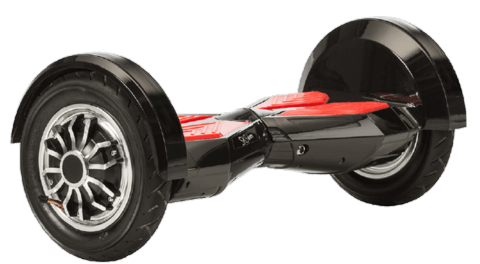
\includegraphics[trim = 0mm 0mm 0mm 0mm, clip,scale=0.4]{imagenes/Balancing_robot/segway}
	\caption{SegWay comercial.}
	\label{fig:segway}
\end{figure}


\begin{definicion}Péndulo: Es un sistema físico que puede oscilar bajo la acción gravitatoria u otra característica física (elasticidad, por ejemplo) y que está configurado por una masa suspendida de un punto o de un eje horizontal fijos mediante un hilo, una varilla, u otro dispositivo que sirve para medir el tiempo. \newline
\end{definicion}
Así, y como el lector podrá imaginar, un péndulo invertido tendrá el aspecto de la figura \ref{fig:pendulo}. 

\begin{figure}[H]
	\center
	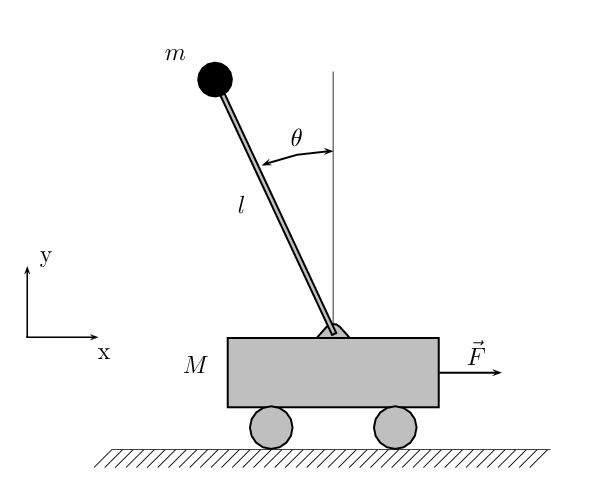
\includegraphics[trim = 0mm 0mm 0mm 0mm, clip,scale=1.6]{imagenes/Balancing_robot/pendulo}
	\caption{Representación péndulo invertido.}
	\label{fig:pendulo}
\end{figure}

Consiste en un péndulo donde el centro de masas se encuentra situado por encima del punto o eje de balanceo. Como cabe esperar, esta disposición dota al sistema de una inestabilidad estática. Recordamos que un sistema es estable cuánto mas cercano esta del plano horizontal de apoyo su centro de gravedad. \newline

El fundamento de este proyecto consistirá por tanto en intentar corregir esta inestabilidad, y forma parte de uno de los problemas mas famosos en cuánto a teoría de control y dinámica de sistemas. 

\newpage
\section{Diseño del sistema}\label{sec:Diseno}

Mediante una comunicación i2c con un sensor IMU, el micro-controlador obtiene el ángulo actual de sistema. Obtenido el ángulo por el micro-controlador una comunicación de tipo serie lo envía a la FPGA, en un formato binario de 1 byte para la parte entera y 1 byte para la parte decimal. Una shield con un driver de motores DC conectada a la FPGA dota a esta de la posibilidad de variar la velocidad y el sentido de dos motores DC que permiten la estabilización del sistema. La velocidad de los motores para una correcta corrección del ángulo se calcula mediante un controlador PD básico implementado en la FPGA.

\begin{center}
	\begin{figure}[H]
		\center
		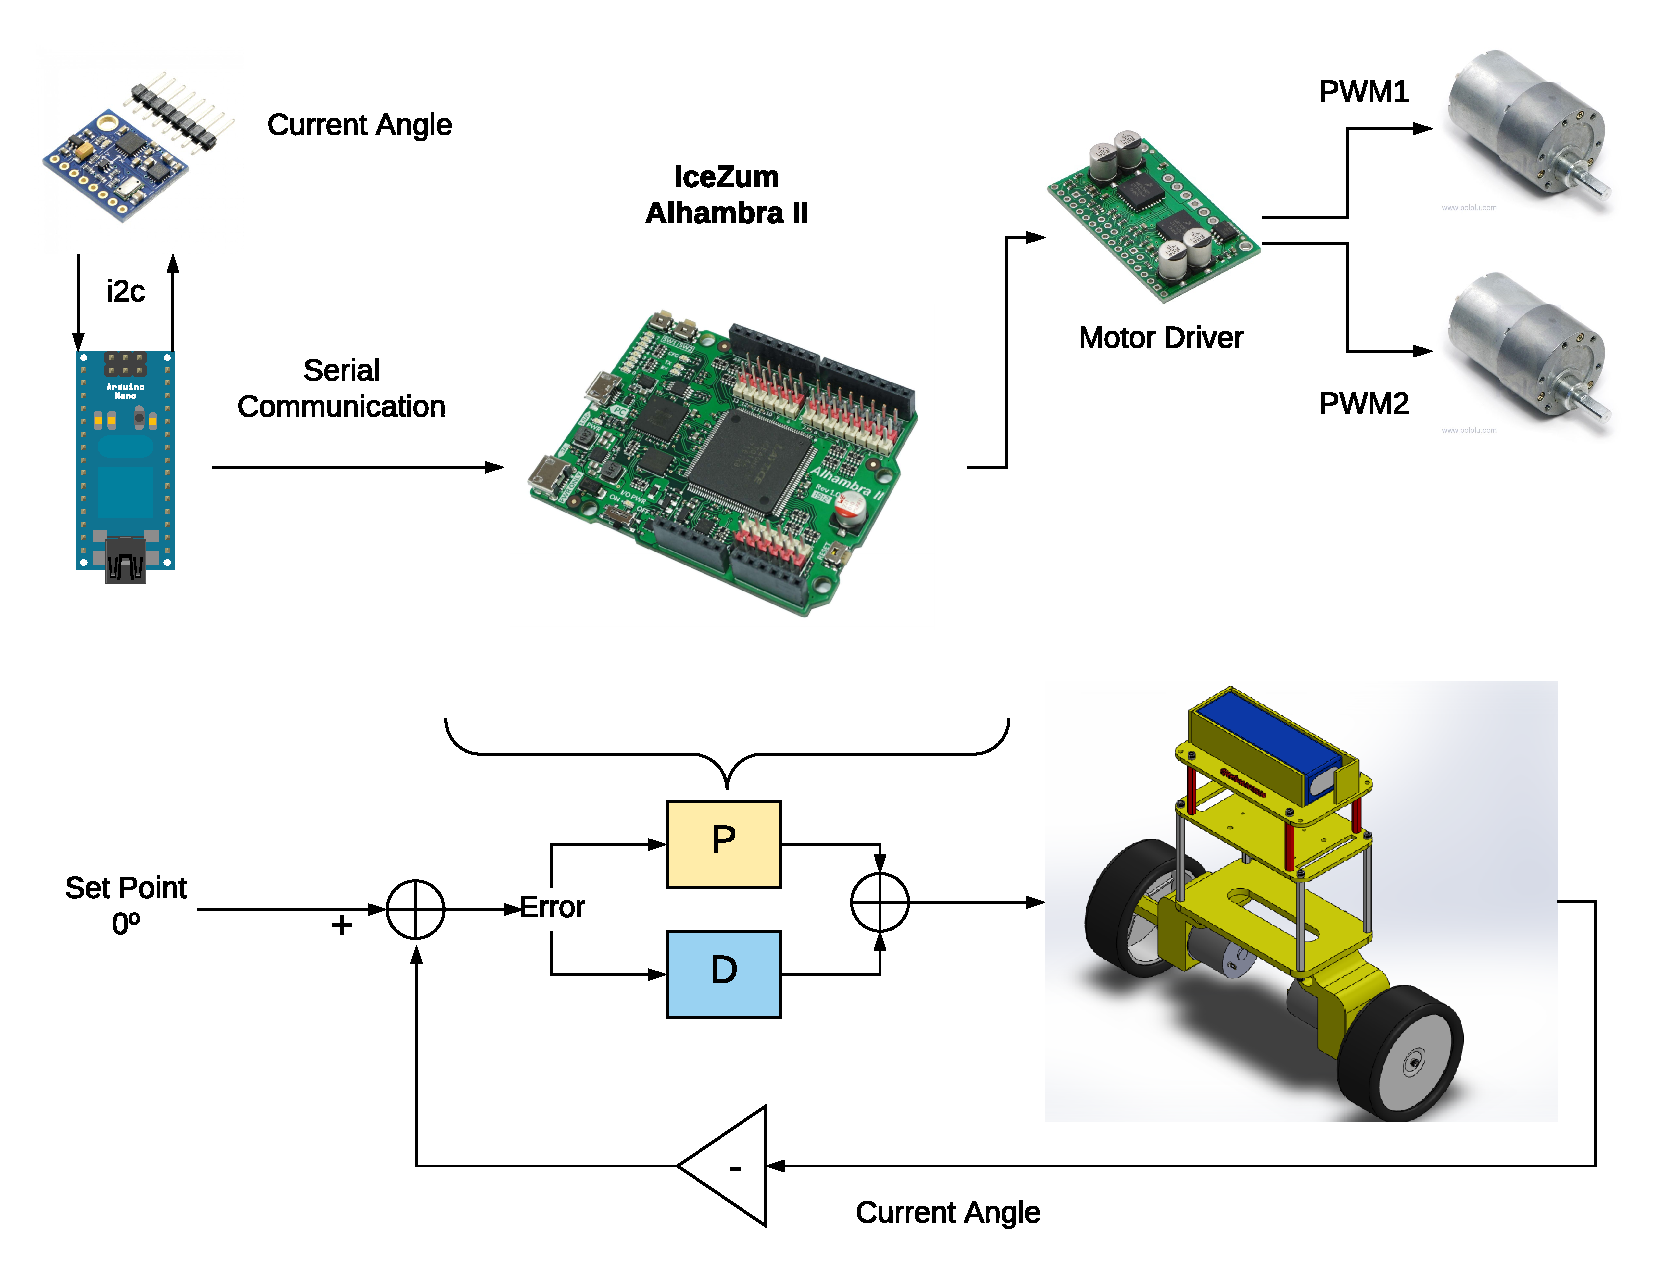
\includegraphics[trim = 0mm 0mm 0mm 0mm,clip, angle=0, scale = 0.6]{imagenes/Balancing_Robot/final.pdf}
		\caption{Diagrama de bloques final.}
		\label{fig:final}
	\end{figure}
\end{center}

%En esta sección se propone una solución al problema planteado proporcionando esta con un alto nivel de abstracción. En la sección \ref{sec:Implementacion} se profundizará aún más en los detalles de los diferentes sub-sistemas que aquí se exponen.

En los sucesivos capítulos se irá profundizando en cada uno de los bloques anteriores que forman la solución final (figura \ref{fig:final}). 


\newpage
\section{Implementación del sistema}\label{sec:Implementacion}
\subsection{Fabricación estructura mecánica (Física de un Balancing Robot)}
Teniendo en cuenta la física de un balancing robot y con el objetivo por tanto de solucionar el problema clásico del péndulo invertido, se propone la estructura mecánica de las figuras \ref{fig:EnsanBalanceFront}, \ref{fig:EnsanBalanceLateral} y \ref{fig:EnsanBalanceCab}, diseñadas con SolidWorks[] y a partir de la cuál se ensamblarán el resto de los componentes.

\begin{center}
	\begin{figure}[H]
		\center
		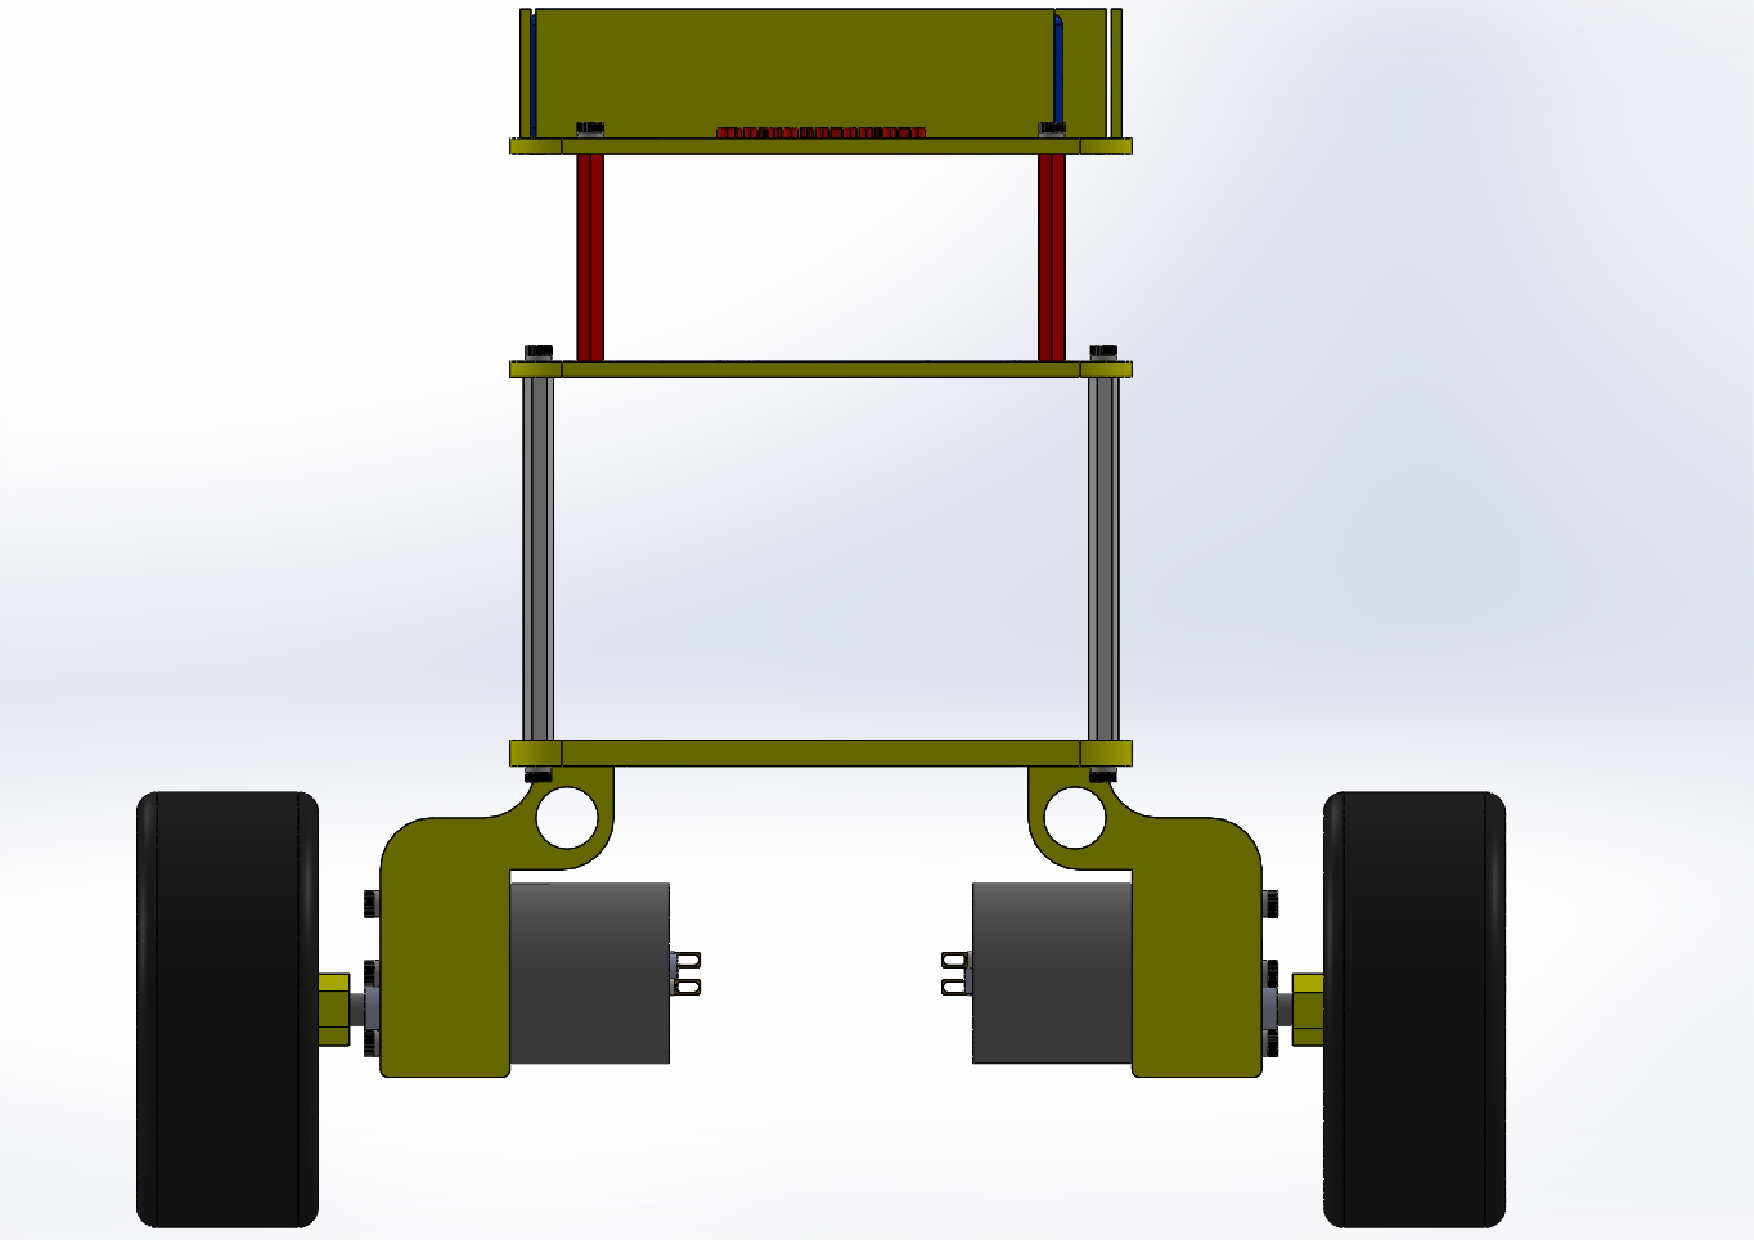
\includegraphics[trim = 1cm 0mm 2.7cm 0mm,clip, angle=0, scale = 0.4]{imagenes/Balancing_Robot/EnsanBalanceFront.PDF}
		\caption{Vista frontal Balancing Robot.}
		\label{fig:EnsanBalanceFront}
	\end{figure}
\end{center}

\begin{center}
	\begin{figure}[H]
		\center
		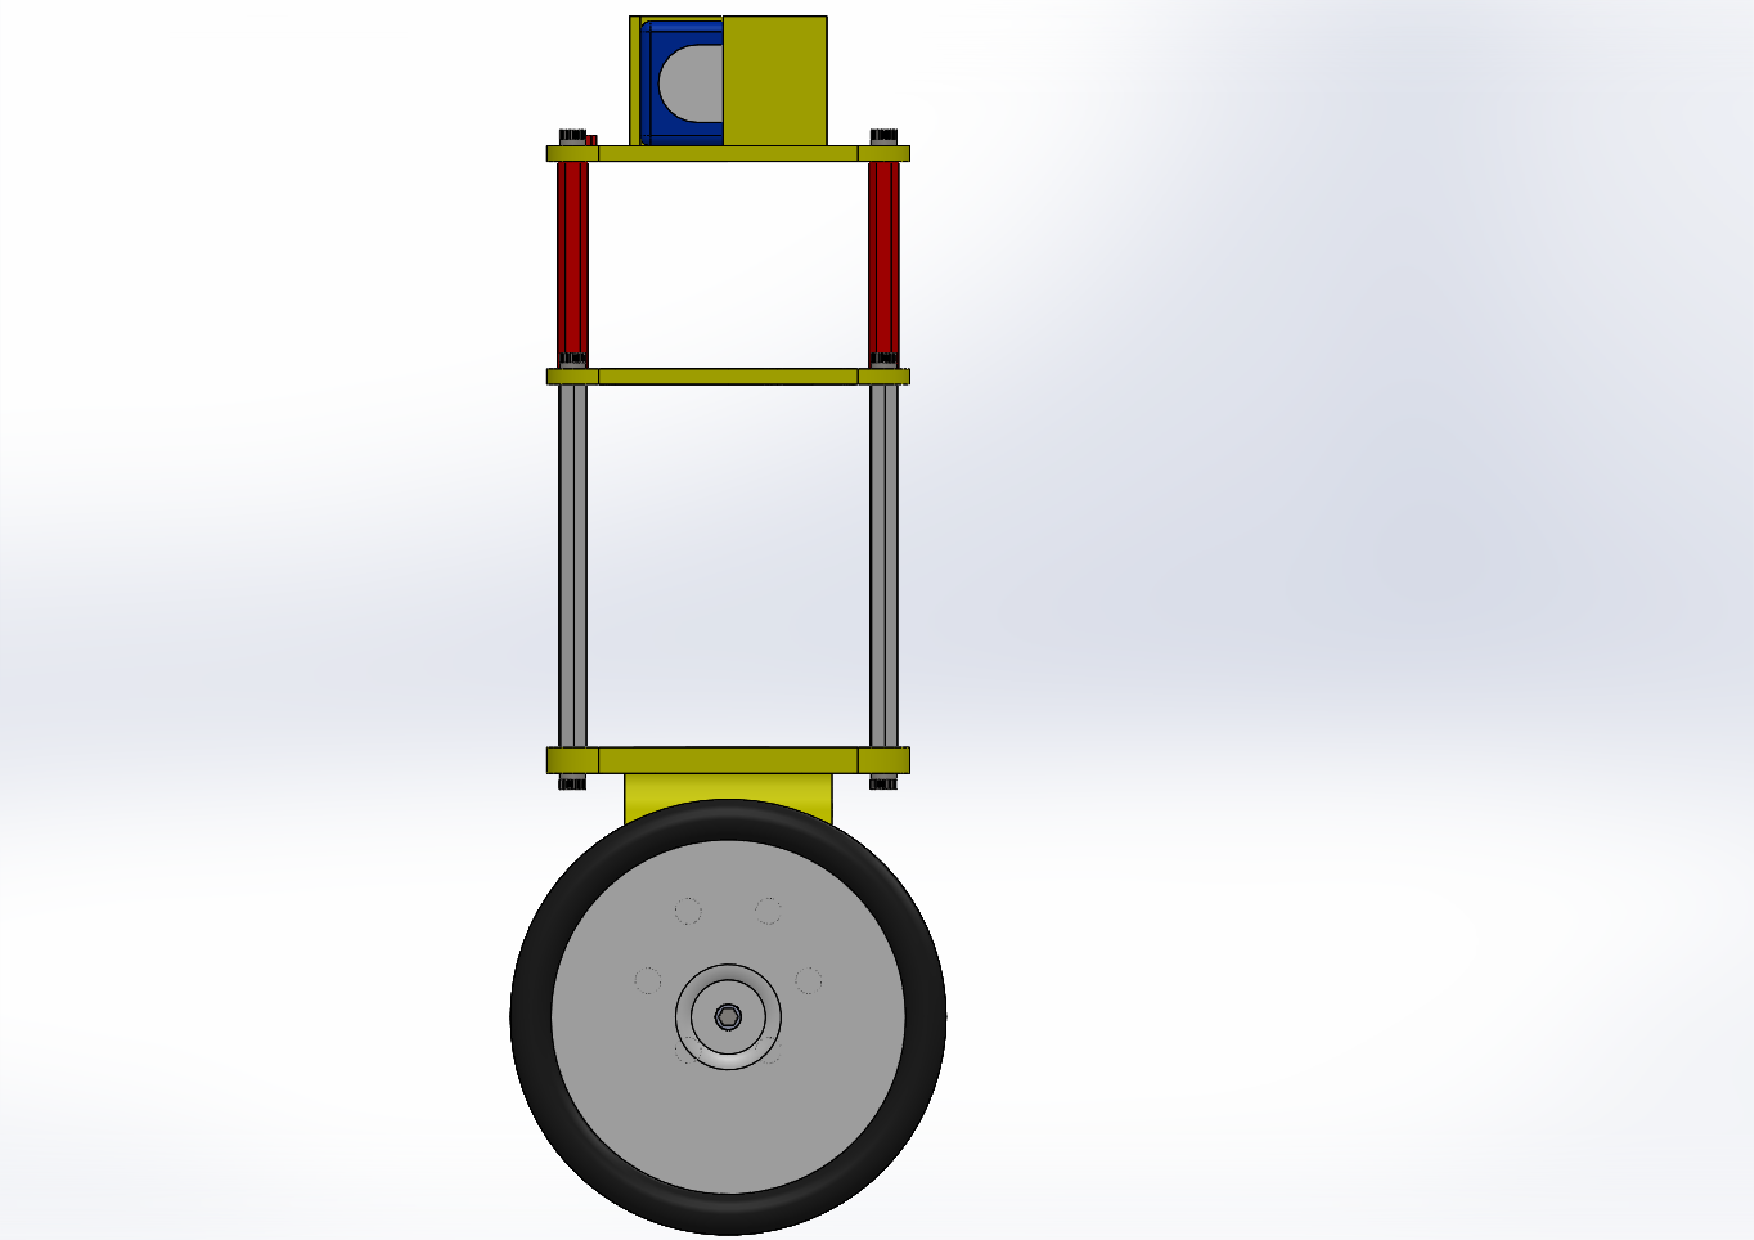
\includegraphics[trim = 5cm 0mm 10cm 0mm,clip, angle=0, scale = 0.5]{imagenes/Balancing_Robot/EnsanBalanceLateral.PDF}
		\caption{Vista lateral derecha Balancing Robot.}
		\label{fig:EnsanBalanceLateral}
	\end{figure}
\end{center}

\begin{center}
	\begin{figure}[H]
		\center
		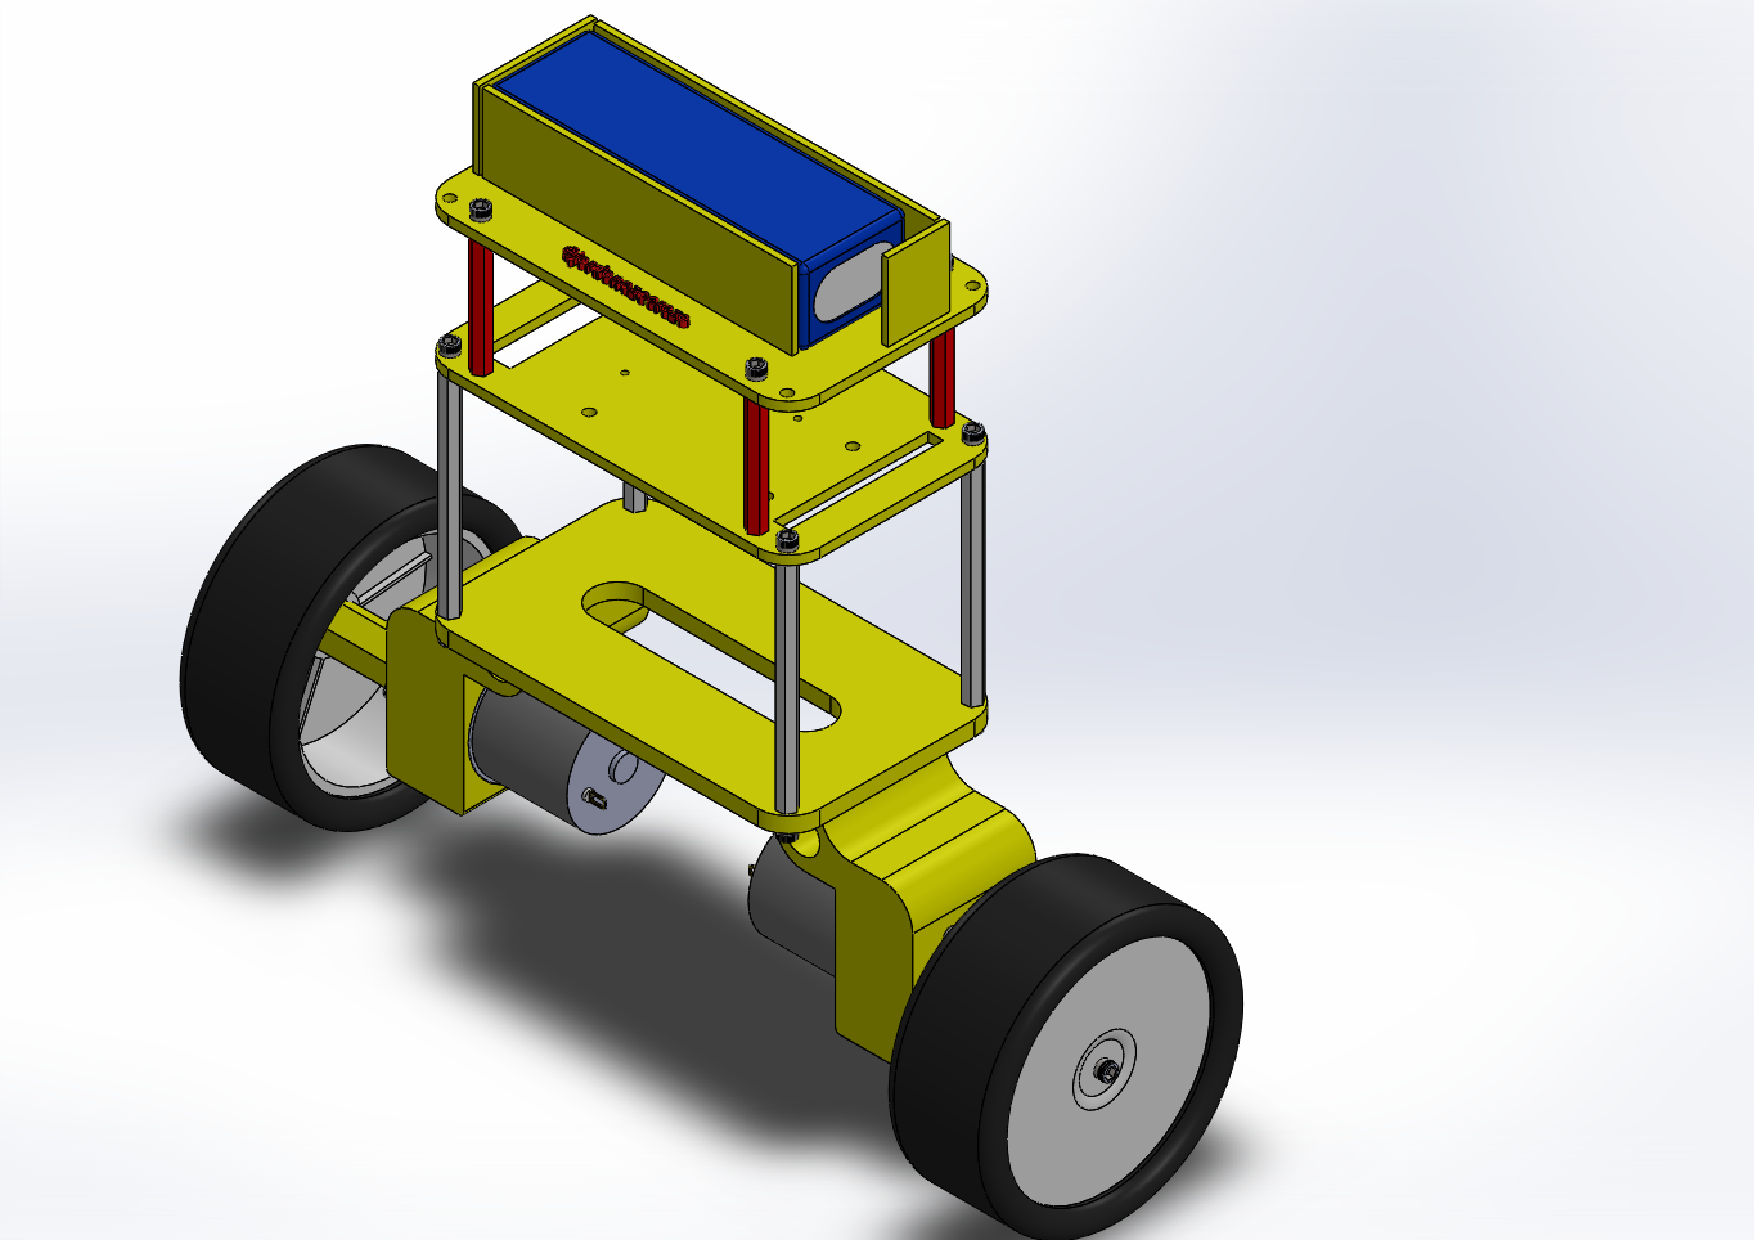
\includegraphics[trim = 20mm 0mm 8cm 0mm,clip, angle=0, scale = 0.5]{imagenes/Balancing_Robot/EnsanBalanceCab.PDF}
		\caption{Perspectiva Balancing Robot.}
		\label{fig:EnsanBalanceCab}
	\end{figure}
\end{center}

Se tienen en cuenta diferentes aspectos en el diseño de esta estructura que se relacionan directamente con la física de un Robot Balancín y con ello, del péndulo invertido. \newline
Como se argumenta en la sección \ref{sec:Descripcion_balancin}, un sistema en reposo es estable cuando mas cercano esta del plano horizontal su centro de masas. Si se tiene en cuenta que la naturaleza del sistema planteado es inherentemente inestable, se hace necesario conocer el mejor punto donde debe estar el centro de masas para permitir una mejor estabilización. \newline

Asumiendo la caracterización del modelado matemático en [][][], se asume por tanto que para conseguir una mayor facilidad en la estabilización, el centro de masas debe estar colocado por encima del punto medio del eje vertical de nuestro sistema. Por lo tanto, se ha de tener en cuenta el peso de todos los componentes para una colocación tal que permita lo anterior. \newline
En la figura \ref{fig:center_mass} se representa el cálculo con SolidWorks de este centro de masas donde sólo se han tenido en cuenta los elementos más pesados del sistema final, esto es, motores DC, batería, estructura mecánica y ruedas. 

\begin{figure}[H]
	\center
	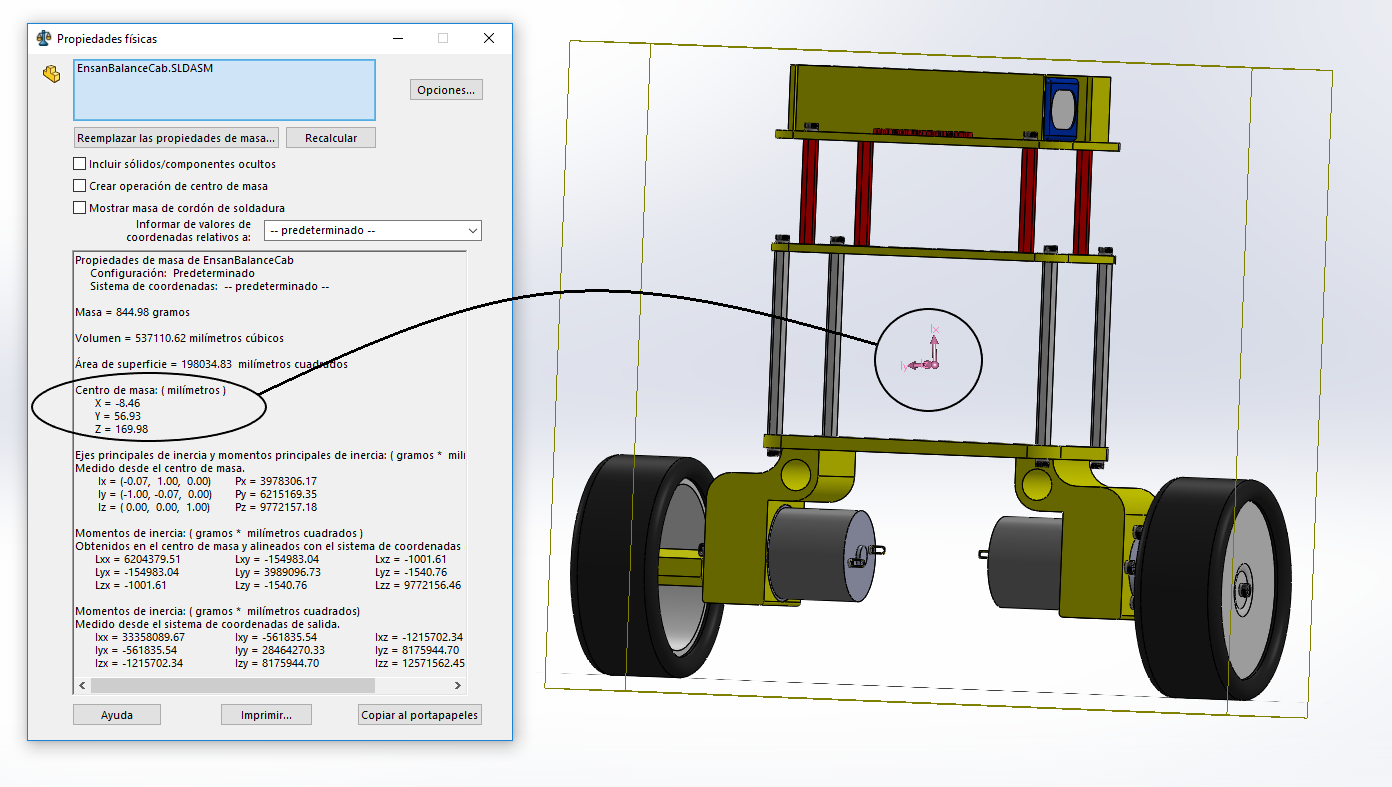
\includegraphics[scale=0.4]{imagenes/Balancing_robot/center_mass}
	\caption{Centro de masas en sistema final.}
	\label{fig:center_mass}
\end{figure}

\subsection{Unidad de medida inercial MPU6050 en Arduino Nano}\label{sec:MPU6050}

Es necesario un conocimiento constante del ángulo del sistema para su posterior análisis y corrección, para ello se hace uso del MPU6050 conectado mediante una comunicación I2C a un Arduino Nano. \newline

El MPU6050[] es una unidad de medida inercial (Inertial Measure Unit, IMU )con 6 grados de libertad (6DOF) fabricado por Invensense[]. Cuenta con un acelerómetro y giroscopio y permite una comunicación tanto por SPI como por bus I2C. Para corregir algunos de los problemas de captación de datos planteados en \ref{sec:IMU} incorpora un procesador interno (Digital Motion Processor, DMP) que ejecuta algoritmos de fusión de datos (Motion Fusion) para combinar las mediciones de los sensores internos evitando tener que realizar los filtros de forma exterior.\newline

Debido a su bajo precio y gran calidad es uno de los IMUs más utilizados en la actualidad.
En la figura \ref{fig:IMU1} se muestra una imagen del MPU6050

\begin{figure}[H]
	\center
	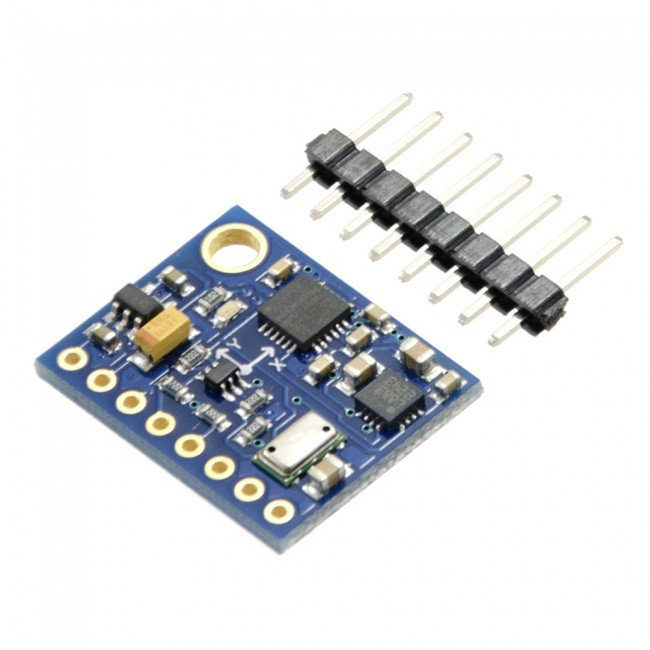
\includegraphics[scale=0.2]{imagenes/Balancing_robot/IMU1}
	\caption{MPU6050 IMU.}
	\label{fig:IMU1}
\end{figure}
\subsubsection{Pin out}

En la figura \ref{fig:MPU6050_schematic} se muestra el diagrama esquemático de conexiones del MPU6050.

\begin{figure}[H]
	\center
	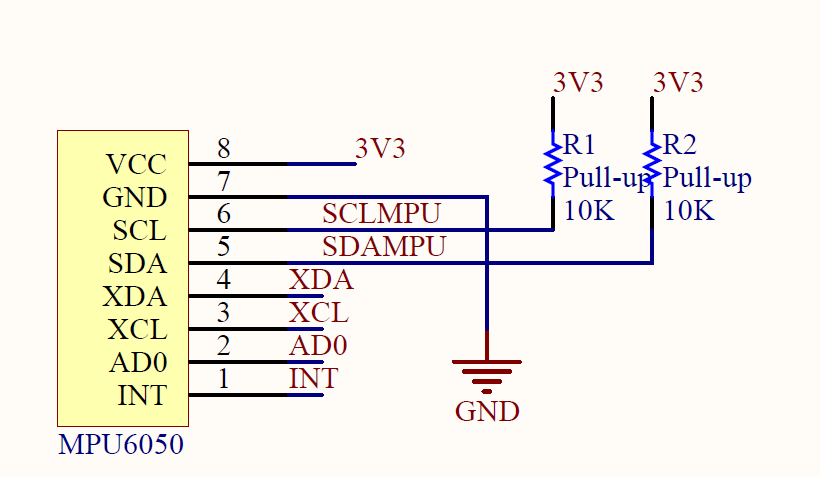
\includegraphics[scale=0.4]{imagenes/Balancing_robot/MPU6050_schematic}
	\caption{MPU6050 IMU.}
	\label{fig:MPU6050_schematic}
\end{figure}

Tiene una tensión de alimentacion de 3.3V. El pin de reloj para la conexión I2C (Serial Clock Line, SCL) y el pin de datos (Serial Data Line, SDA) representan la conexión para el bus con Arduino Nano. El pin AD0 permite al usuario final cambiar la dirección del MPU (slave) la cuál por defecto es 0x68h conectado a GND. Si se conecta a Vcc la dirección cambia a 0x69h. El pin INT produce una señal en alta cuando el dato en cuestión está disponible por parte del MPU para ser capturado, y avisará por medio de una interrupción al Arduino Nano con el fin de poder ser obtenido. \newline

\subsubsection{Programa para Arduino nano}
Para la implementación en Arduino Nano se utiliza la librería desarrollada por Jeff Rowberg []. La razón del uso de esta librería es debido a que incorpora la utilización del DMP cuyas ventajas en este caso se representan en la figura \ref{fig:coexistencia1}\newline

\begin{figure}[H]
	\center
	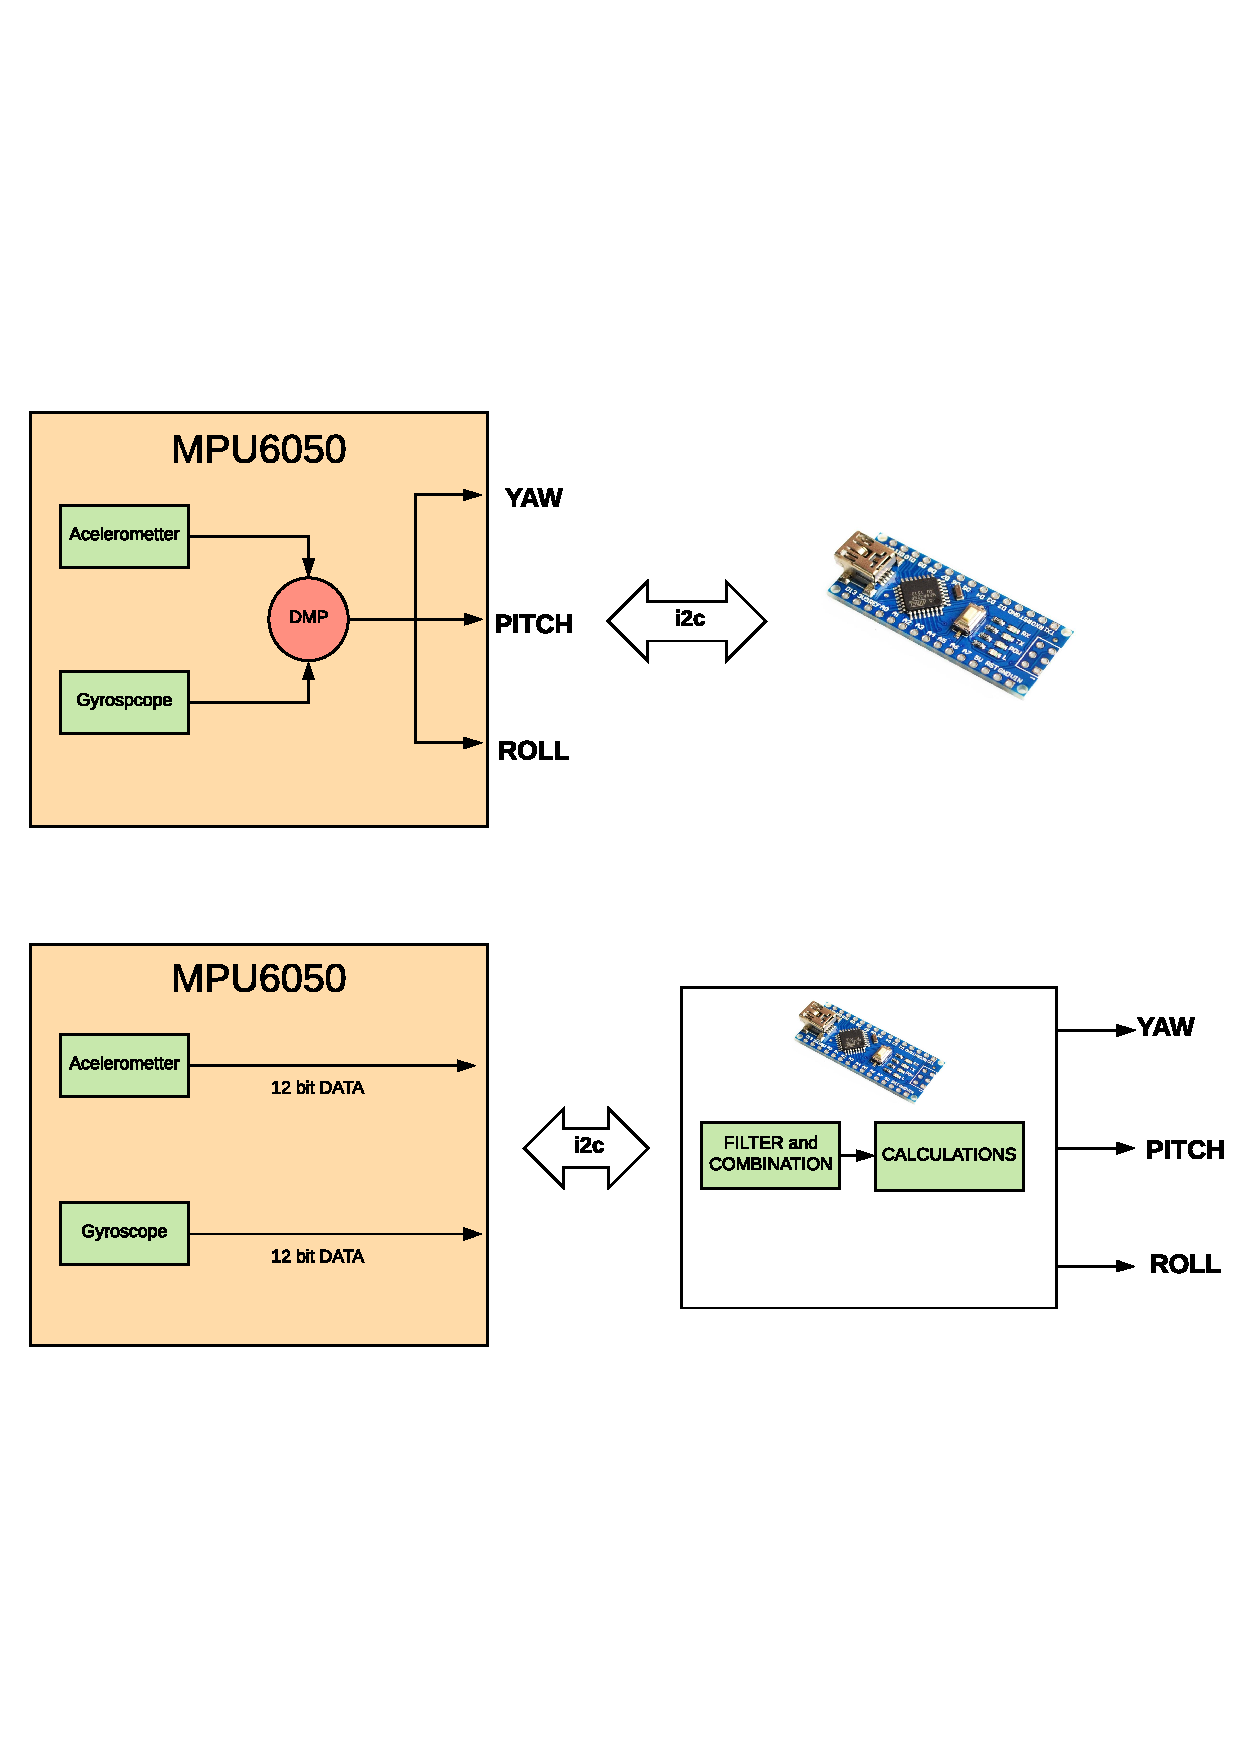
\includegraphics[trim = 0mm 4cm 0mm 2cm, clip,scale=0.6]{imagenes/Balancing_robot/DMPexample.pdf}
	\caption{Ventaja de uso en la utilización de DMP.}
	\label{fig:coexistencia1}
\end{figure}

\subsubsection{Valores del sensor. DMP. }

Los valores 


\subsection{Implementación PCB}

Después de caracterizar todo el sistema, y teniendo en cuenta el diagrama de conexiones necesario no solo entre el micro-controlador y FPGA sino también para el módulo de cámara OV7670 y el driver del motor, es conveniente y apropiado un circuito impreso que resolviese algunos problemas de ruido, cables excesivos, etc. \newline

El circuito impreso alberga los siguientes componentes y
comportamientos:

\begin{itemize}
	\item Un total de 28 pines en la parte exterior de la PCB y dispuestos en la posición correcta para un encaje en la placa IceZum Alhambra II (figura \ref{fig:pin_headers}), lo cuál permite poder usar como entradas o salidas los pines de la FPGA. Para conocer la posición exacta de los pines en la placa se hizo uso del proyecto en Altium el cuál está disponible en GitHub.
	
	\begin{figure}[H]
		\center
		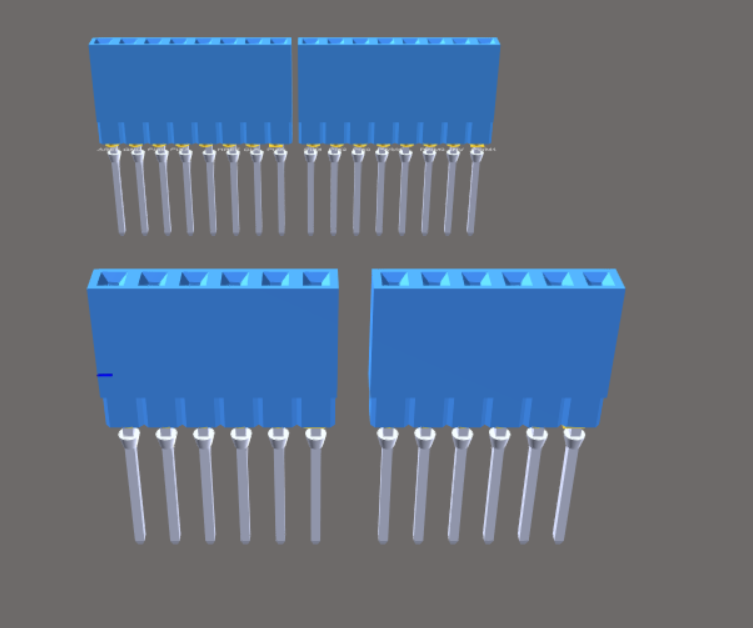
\includegraphics[scale=0.5]{imagenes/Balancing_robot/pin_headers.PNG}
		\caption{Pin headers para IceZum Alhambra II.}
		\label{fig:pin_headers}
	\end{figure}
	
	
	\item 4 conexiones VCC y GND de 12 Voltios para alimentar los ESC de los motores brushless del vehículo aéreo. Para ello se ha elegido el componente de la figura \ref{fig:screw}, por cumplir con las características adecuadas de temperatura máxima a la que puede estar sometido y las cuales serán analizadas más adelante: 
	
	\begin{figure}[H]
		\center
		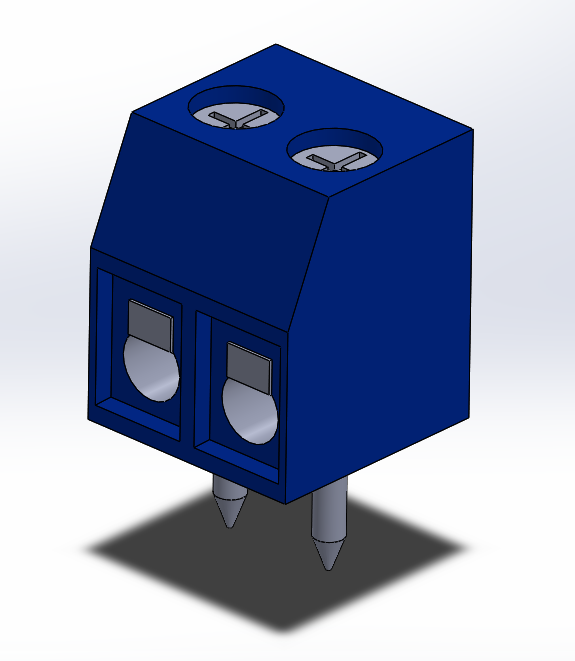
\includegraphics[scale=0.5]{imagenes/Balancing_robot/SCREW.PNG}
		\caption{Conector GND y VCC.}
		\label{fig:screw}
	\end{figure}
	
	
	\item Una conexión VCC y GND para alimentar las anteriores conexiones. Este conector irá directo a una batería LIPO de 11.1V (3 celdas) y 2200mAh. El hecho de elegir esta batería viene dado al voltaje mínimo por el que se alimentan los ESCs de los motores brushless así como los motores y el driver del motor utilizado para el Balancing-robot. Un análisis mas detallado de la batería puede encontrarse en subsección \ref{sec:Bateria}
	
	\item Módulo de pines "header" para la conexión del MPU6050 anteriormente descrito (figura \ref{fig:mpu6050_connector).
		
		\begin{figure}[H]
			\center
			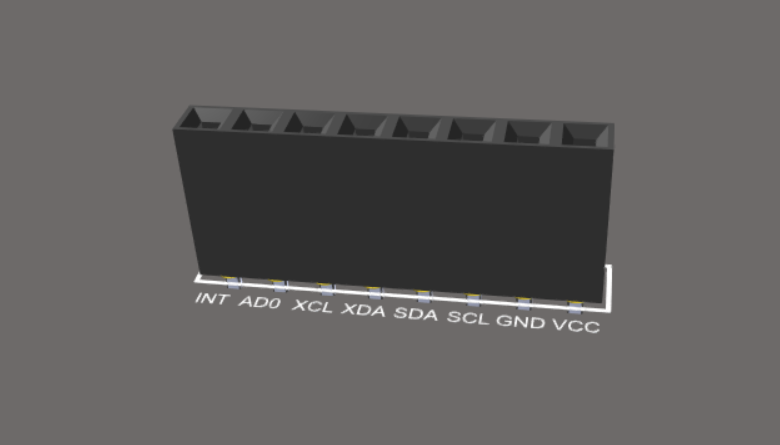
\includegraphics[scale=0.5]{imagenes/Balancing_robot/mpu6050_connector.PNG}
			\caption{Módulo MPU6050.}
			\label{fig:mpu6050_connector}
		\end{figure}
		
		
		\item Se hace una extensión de los pines mas importantes del MPU6050 para que puedan ser utilizados por el micro-controlador en caso de que el análisis del ángulo, como en este proyecto, forme parte de un proceso gobernado por dicho micro-controlador.
		
		\item Se dispone para el usuario final la posibilidad de unos "jumpers" (figura \ref{fig:jumpers}) para dar la opción al usuario sobe quién gobernará la comunicación I2C, la FPGA o el micro-controlador, para el cuál se podrán usar los conectores del apartado anterior.\newline
		
		\begin{figure}[H]
			\center
			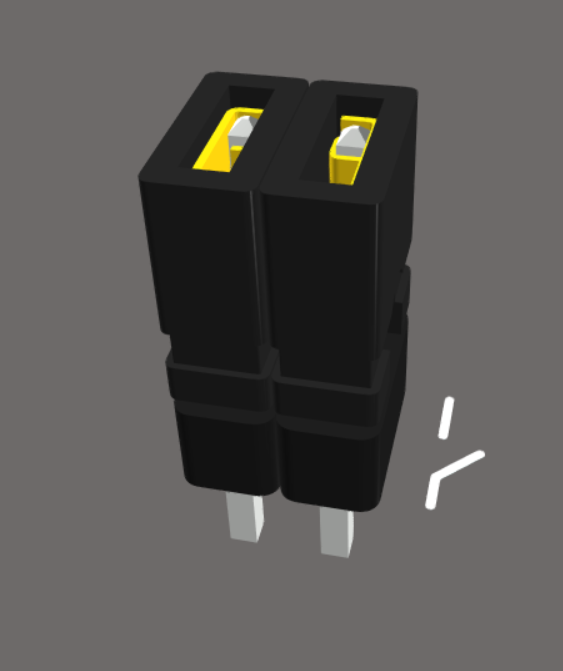
\includegraphics[scale=0.5]{imagenes/Balancing_robot/jumpers.PNG}
			\caption{Jumpers para configuración i2c MPU6050.}
			\label{fig:jumpers}
		\end{figure}
		
		
		Al albergar una línea de datos no se hace necesario tener en cuenta las características térmicas del conector en cuestión, y al trabajar a una frecuencia relativamente pequeña, puede aceptarse el ruido que los "jumpers" pudiesen introducir en la comunicación I2C.
		
		\item Gran parte de los micro-controladores actuales trabajan a 3.3-5v pero la tensión de entrada que soportan puede llegar hasta 12V, por lo que se aprovecha la alimentación de la batería LIPO y se implementa un nuevo conector con dos pin "header" a VCC y GND que alimentarán el micro-controlador.
		
		\item Un módulo que pueda albergar la cámara OV7670 formado por pin "headers" de tipo macho y cada uno de los cuales estará unido a uno de los pines in-out de la FPGA, como se verá mas adelante en el esquemático general. 
		
		\item Un módulo que pueda albergar el driver del motor DC utilizado en este caso y que permita la conexión directa con los pines de la IceZum Alhambra II, pues por ejemplo la señal pwm que definirá la velocidad de los motores será una salida por uno de los pines de la FPGA, y deberá ser una entrada al driver del motor.
		
		\item Para que no haya errores en la transmisión I2C se dispone en cada línea una resistencia de pull-up de 4,7K$\Omega$.
	\end{itemize}
	
	En las figuras \ref{fig:top_3D}, \ref{fig:bottom_3D}, \ref{fig:Vista3D1}, \ref{fig:Vista3D2} se incluye una representación en 3D del sistema final con todos los componentes añadidos.
	
	\begin{center}
		\begin{figure}[H]
			\center
			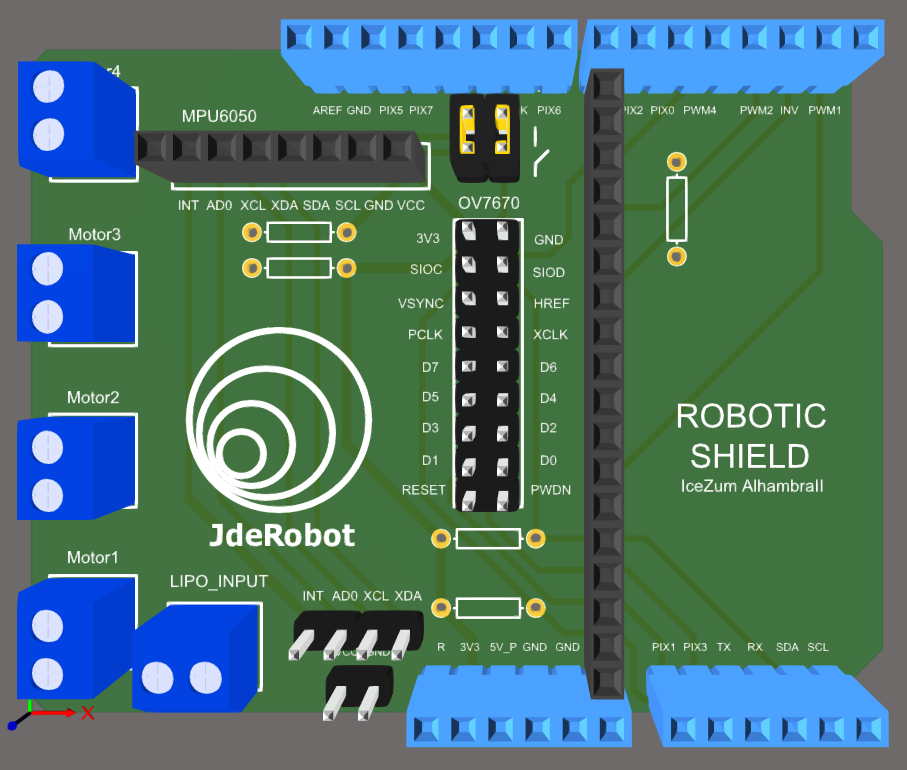
\includegraphics[scale=0.6]{imagenes/Balancing_Robot/top_3D.PNG}
			\caption{}
			\label{fig:top_3D}
		\end{figure}
	\end{center}
	
	\begin{center}
		\begin{figure}[H]
			\center
			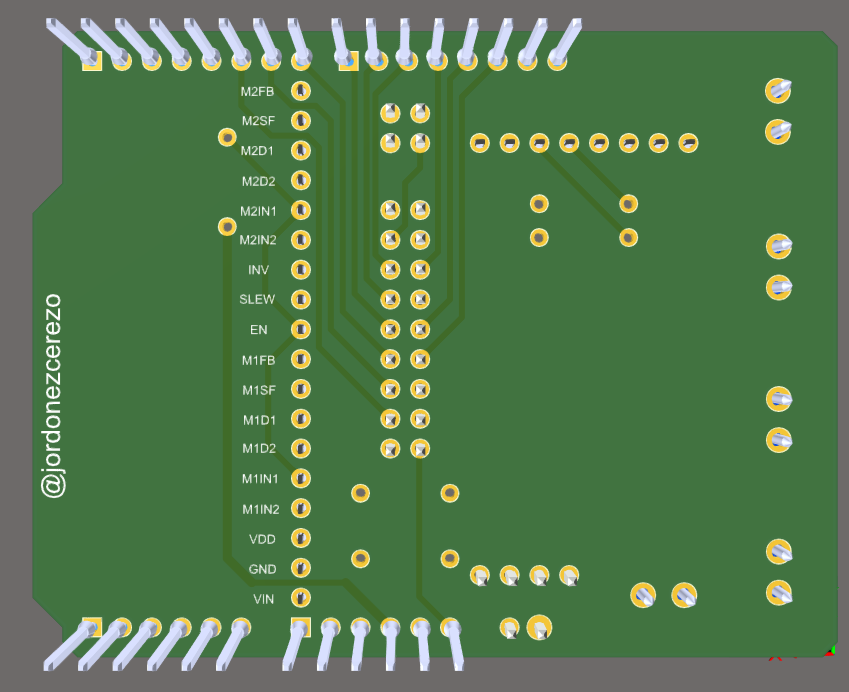
\includegraphics[scale=0.6]{imagenes/Balancing_Robot/bottom_3D.PNG}
			\caption{}
			\label{fig:bottom_3D}
		\end{figure}
	\end{center}
	
	\begin{center}
		\begin{figure}[H]
			\center
			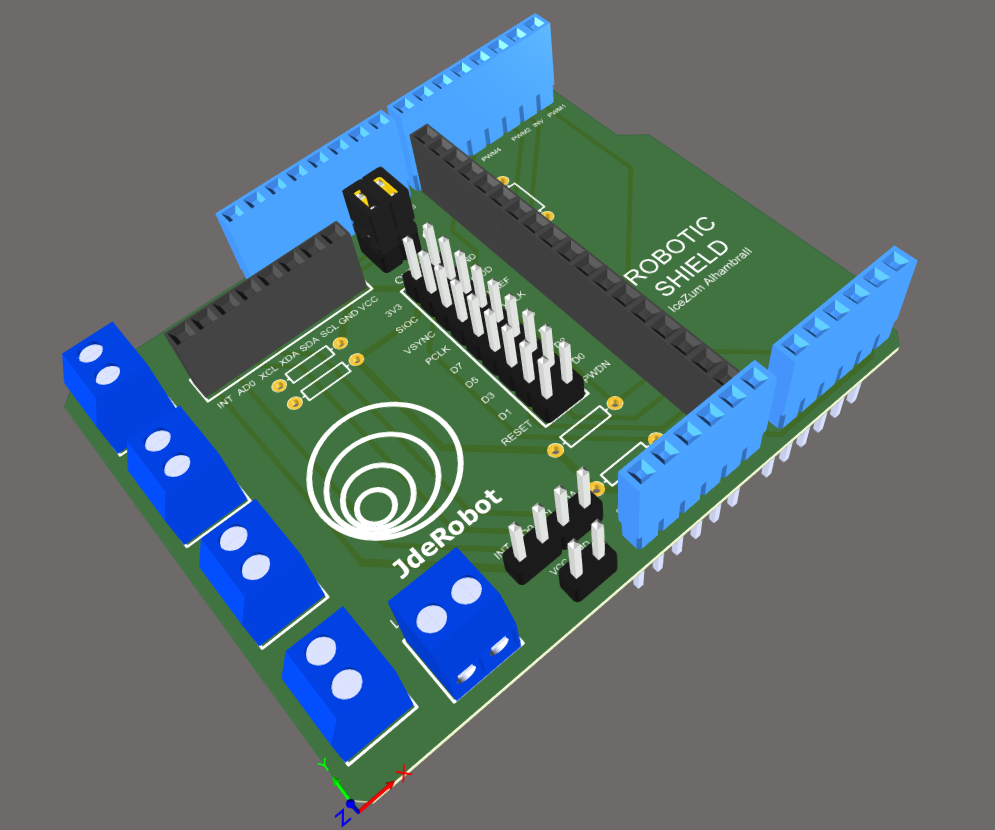
\includegraphics[scale=0.8]{imagenes/Balancing_Robot/Vista3D1.PNG}
			\caption{}
			\label{fig:Vista3D1}
		\end{figure}
	\end{center}
	
	\begin{center}
		\begin{figure}[H]
			\center
			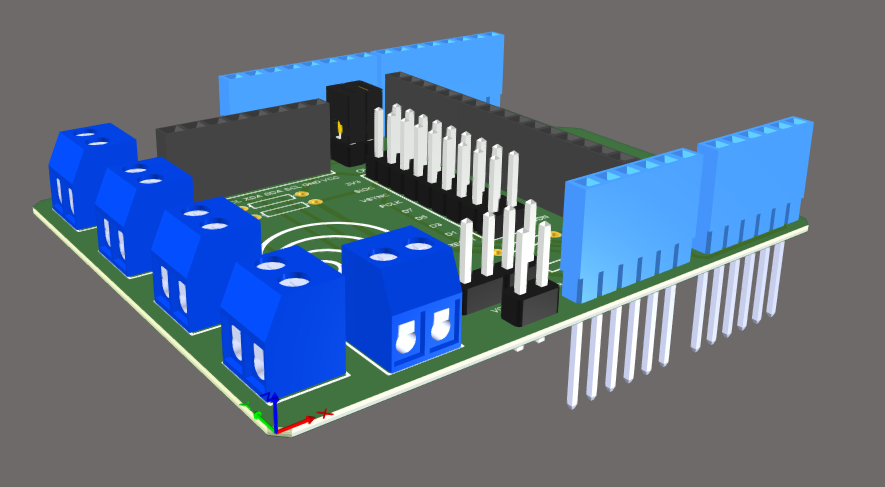
\includegraphics[scale=0.8]{imagenes/Balancing_Robot/Vista3D2.PNG}
			\caption{}
			\label{fig:Vista3D2}
		\end{figure}
	\end{center}


Para el desarrollo de una PCB con los requerimientos descritos en la sección \ref{sec:DisenoPCB} se ha utilizado Altium Designer. El proceso de la elaboración de una PCB en Altium puede ser diferente dependiendo del usuario final, pero en este proyecto se ha seguido la siguiente hoja de ruta:

\begin{itemize}
	\item 1) En primera instancia se crea el proyecto en cuestión.
	\item 2) Para cada componente utilizado se crea una nueva librería formada por el esquemático (Schematic) y por el layout en la pcb (footprint).
	\item 3) Una vez todas las librerías creadas se diseña el esquemático de la placa final, teniendo especial cuidado en que las conexiones sean las adecuadas.
	\item 4) Con el esquemático ya creado, se puede implementar la pcb, definiendo sus bordes, las pistas, los pads, etc.
\end{itemize}

El esquemático es representado en la figura \ref{fig:schematics_tfg}: 
\newpage

\begin{center}
	\begin{figure}[H]
		\center
		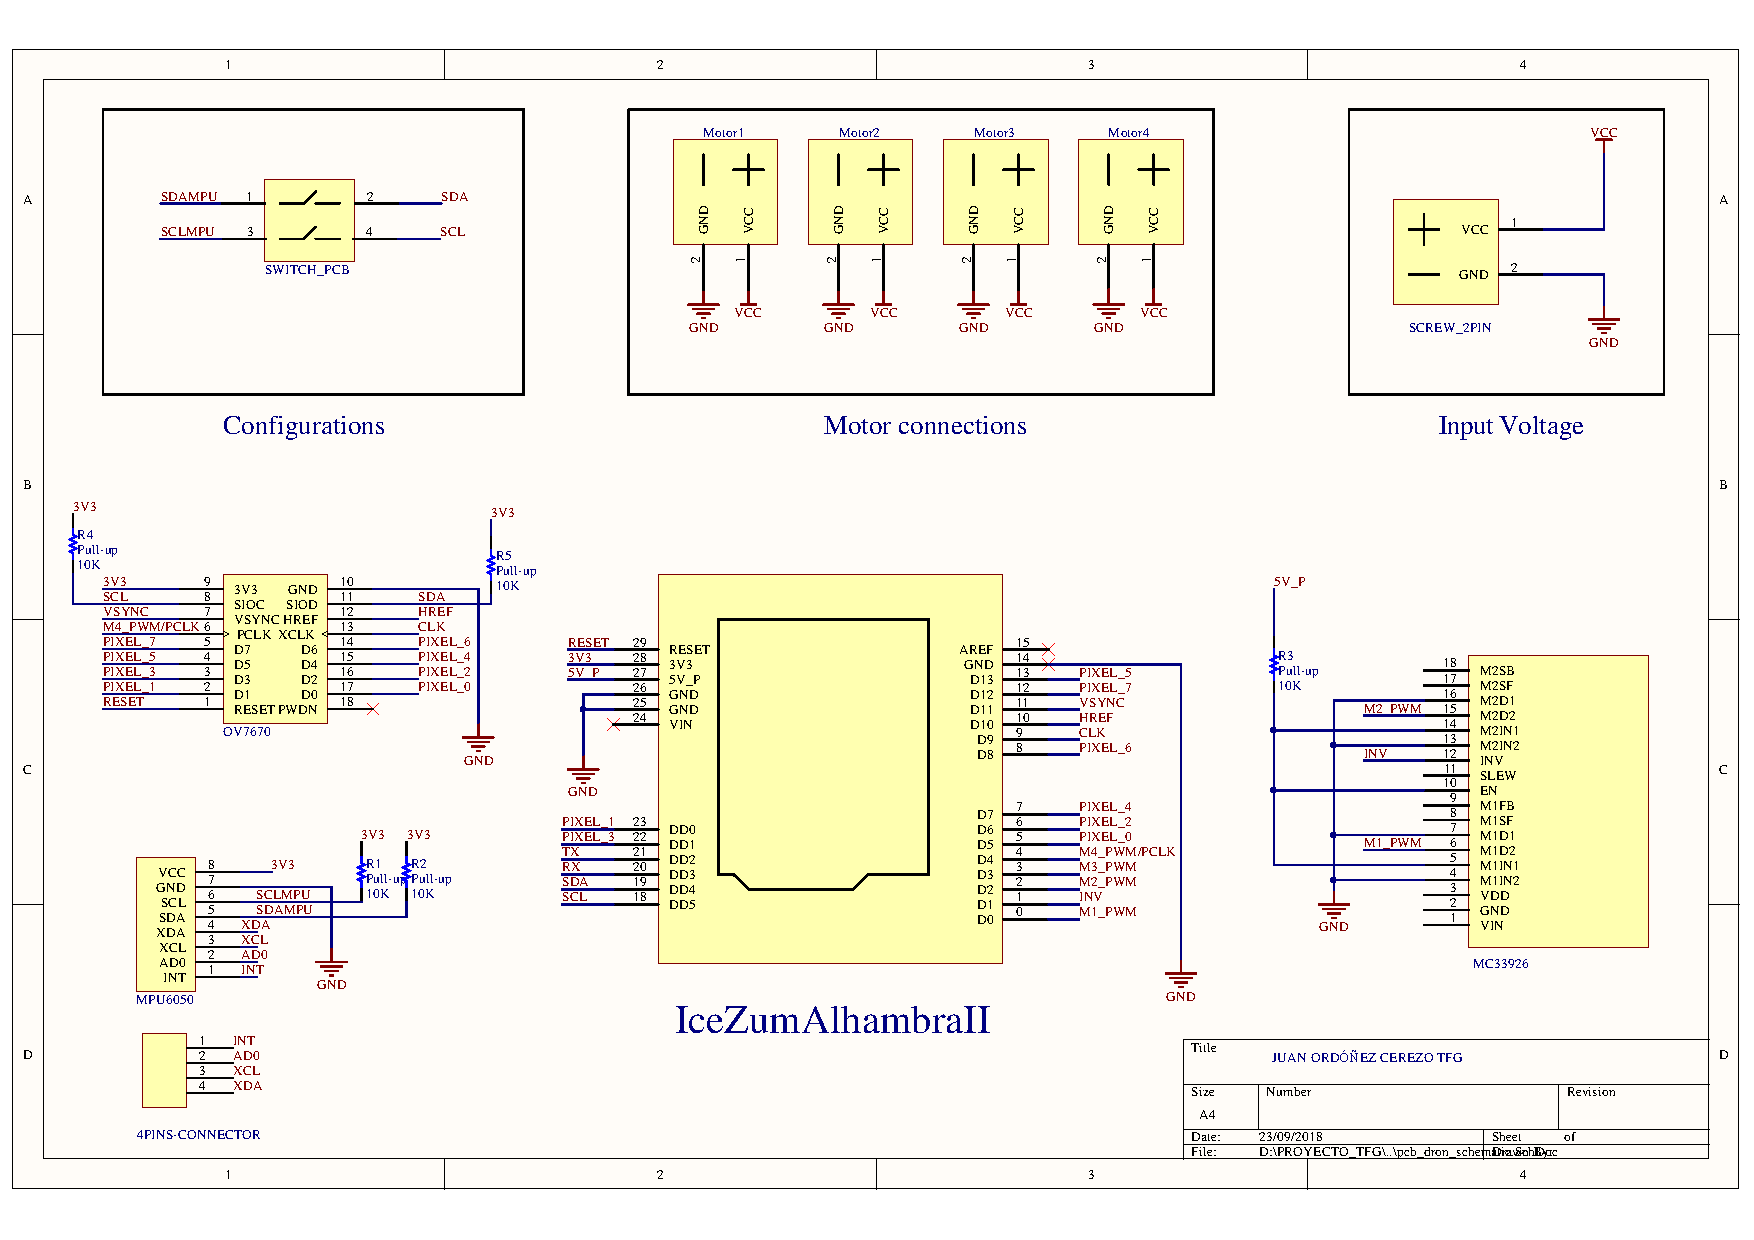
\includegraphics[scale=0.8, angle=90]{imagenes/Balancing_Robot/pcb_dron_schematic.pdf}
		\caption{}
		\label{fig:schematics_tfg}
	\end{figure}
\end{center}
\newpage

\textbf{Tamaño de pista: } \newline
A la hora del diseño de la PCB hay que tener en cuenta el tamaño de las pistas de cobre, sobre todo si por estas la corriente puede ser muy elevada. De no ser así, la PCB podría sufrir daños o llegar incluso a quemarse. \newline

Para calcular un ancho de pista es necesario primero conocer la máxima intensidad que podría circular por ella. Se parte del conocimiento de que uno de los motores del vehículo aéreo no tripulado (este es el peor caso y para el cual es necesario el cálculo de pistas) puede consumir un máximo de 20 amperios. Esta cantidad ha sido extraída del datasheet y suele ser común para este tipo de motores. \newline

La fórmula utilizada para la obtención del ancho de pista ha sido extraída del IPC-2221B, el cual establece los requisitos genéricos para el diseño de tarjetas de circuitos impresos. \newline

Así, la formula se define como en la ecuación \ref{eqn:eqn31}: 

\begin{equation}
I = K * dT^{0.44}*(W*H)^{0.725}
\label{eqn:eqn31}
\end{equation}

Donde: 
\begin{itemize}
	\item I = intensidad máxima en amperios
	\item dT = aumento de temperatura sobre ambiente en ºC
	\item W,H = ancho y grosor en mils
	\item K = 0.024 para pistas internas y 0.048 para externas
\end{itemize}

Se obtienen los siguientes resultados tanto para pistas internas como externas: 

\begin{equation*}
W_{externas} = 18.716 mm 
\end{equation*} 
\begin{equation*}
H_{externas} = 	0.035 mm
\end{equation*}
\begin{equation*}
W_{internas} =  48.6876 mm 
\end{equation*} 
\begin{equation*}
H_{internas} = 	0.035 mm
\end{equation*}

El grosor de la capa es un dato proporcionado por el fabricante. En el presente proyecto se ha utilizado la siguiente web para el pedido de las PCBs: \url{https://www.jlcpcb.com//}. \newline 
El grosor de pista es medido comúnmente en "oz" y en este caso, la empresa fabricante permite una PCB con 1oz de grosor de pista, que equivale a un grosor de 0.035mm.\newline

Si se analizan los resultados obtenidos de la ecuación 3.1 se aprecia claramente la diferencia entre una pista en una capa interna y una pista en una externa. \newline

Una placa de circuito impreso esta dividida en capas, cada una de las capas tiene su función y organizarlas de manera adecuada es una buena práctica para evitar malos comportamientos. Así, una vez analizados los requerimientos, eran necesarias dos capas para la conexión de pines de datos, además siempre es recomendable un plano de tierra en el que todos los pines conectados a GND tengan una capa común. Esto evita ruidos e interferencias además de asegurar una buena referencia de tierra. \newline

En el proveedor de PCBs uttilizado, no hay diferencia de precio entre una PCB de tres capas y una PCB de cuatro capas, así, y considerando que en el mejor de los casos el ancho de pista para los motores "brushless" debe ser de 1.8716cm, se llego a la determinación de la utilización de una de las capas como plano común para las pistas de alimentación de dichos motores. La distribución de las capas será por tanto lo representado en la tabla \ref{tabla:layers_altium}: 

Para el resto de pistas de datos, se asume un ancho de 20mil, que permite una corriente de 1,46 Amperios, más que necesario para esta aplicación


\renewcommand\tablename{Tabla}
\begin{table}[H]
	\centering
	
	\begin{tabular}{|l|l|}
		\hline
		Top Overlay           & Overlay              \\ \hline
		Top Solder            & Solder Mask/Coverlay \\ \hline
		\textbf{Top Layer}    & Signal               \\ \hline
		Dielectric 1          & Dielectric           \\ \hline
		\textbf{VCC}          & Signal               \\ \hline
		Dielectric 2          & Dielectric           \\ \hline
		\textbf{GND}          & Signal               \\ \hline
		Dielectric 4          & Dielectric           \\ \hline
		\textbf{Bottom Layer} & Signal               \\ \hline
		Bottom Solder         & Solder Mask/Coverlay \\ \hline
		Bottom Overlay        & Overlay              \\ \hline
	\end{tabular}
	\caption{Composición de capas en PCB.}
	\label{tabla:layers_altium}
\end{table}



Una imagen en 2D de las capas Top Layer, VCC, GND, Bottom Layer,Top Overlay y Bottom Overlay se representan en la figura \ref{fig:layers_altium}.


\begin{center}
	\begin{figure}[H]
		\center
		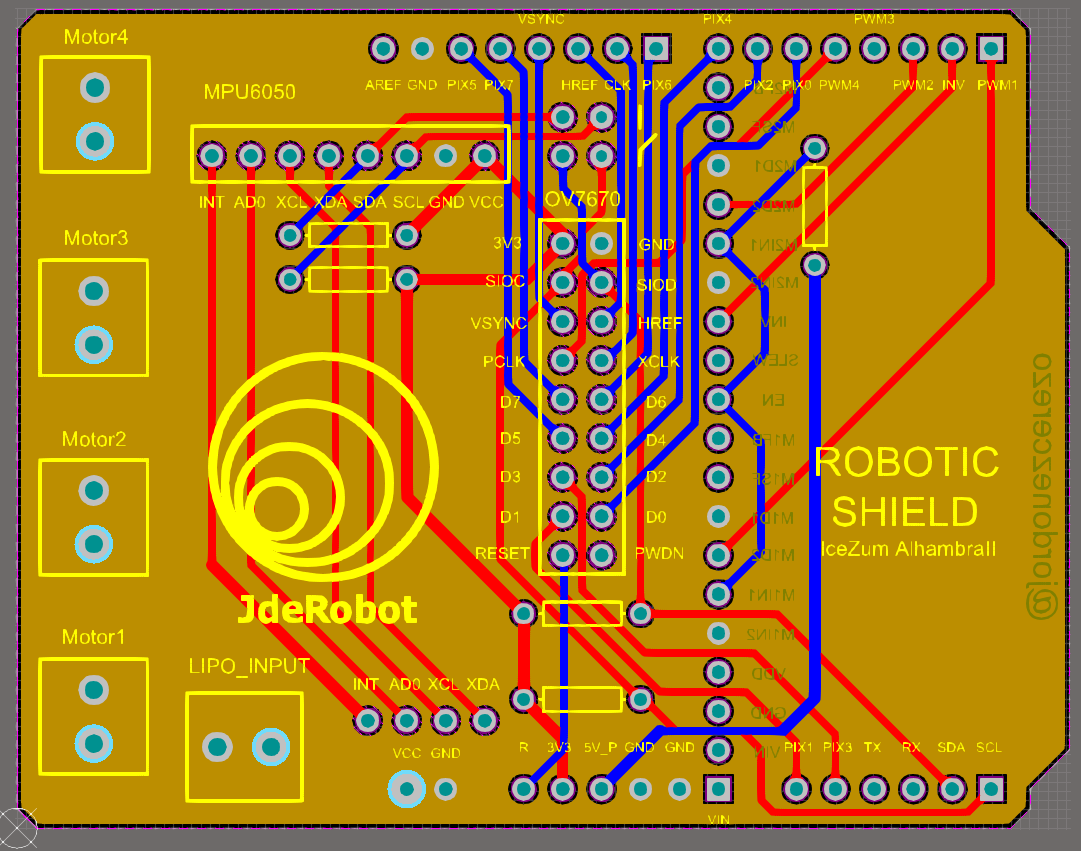
\includegraphics[scale=0.8, angle=90]{imagenes/Balancing_Robot/layers_altium.PNG}
		\caption{}
		\label{fig:layers_altium}
	\end{figure}
\end{center}


\subsection{Implementación IceZum Alhambra-Arduino Nano}\label{sec:Integracion}
El ángulo tiene que ser conocido en la IceZum-Alhambra para la toma de decisiones tanto en dirección como velocidad de los motores. Es necesario por tanto una comunicación micro-controlador/FPGA y que además permita separar procesos secuenciales y paralelos (figura \ref{fig:coexistencia1}).

\begin{figure}[H]
	\center
	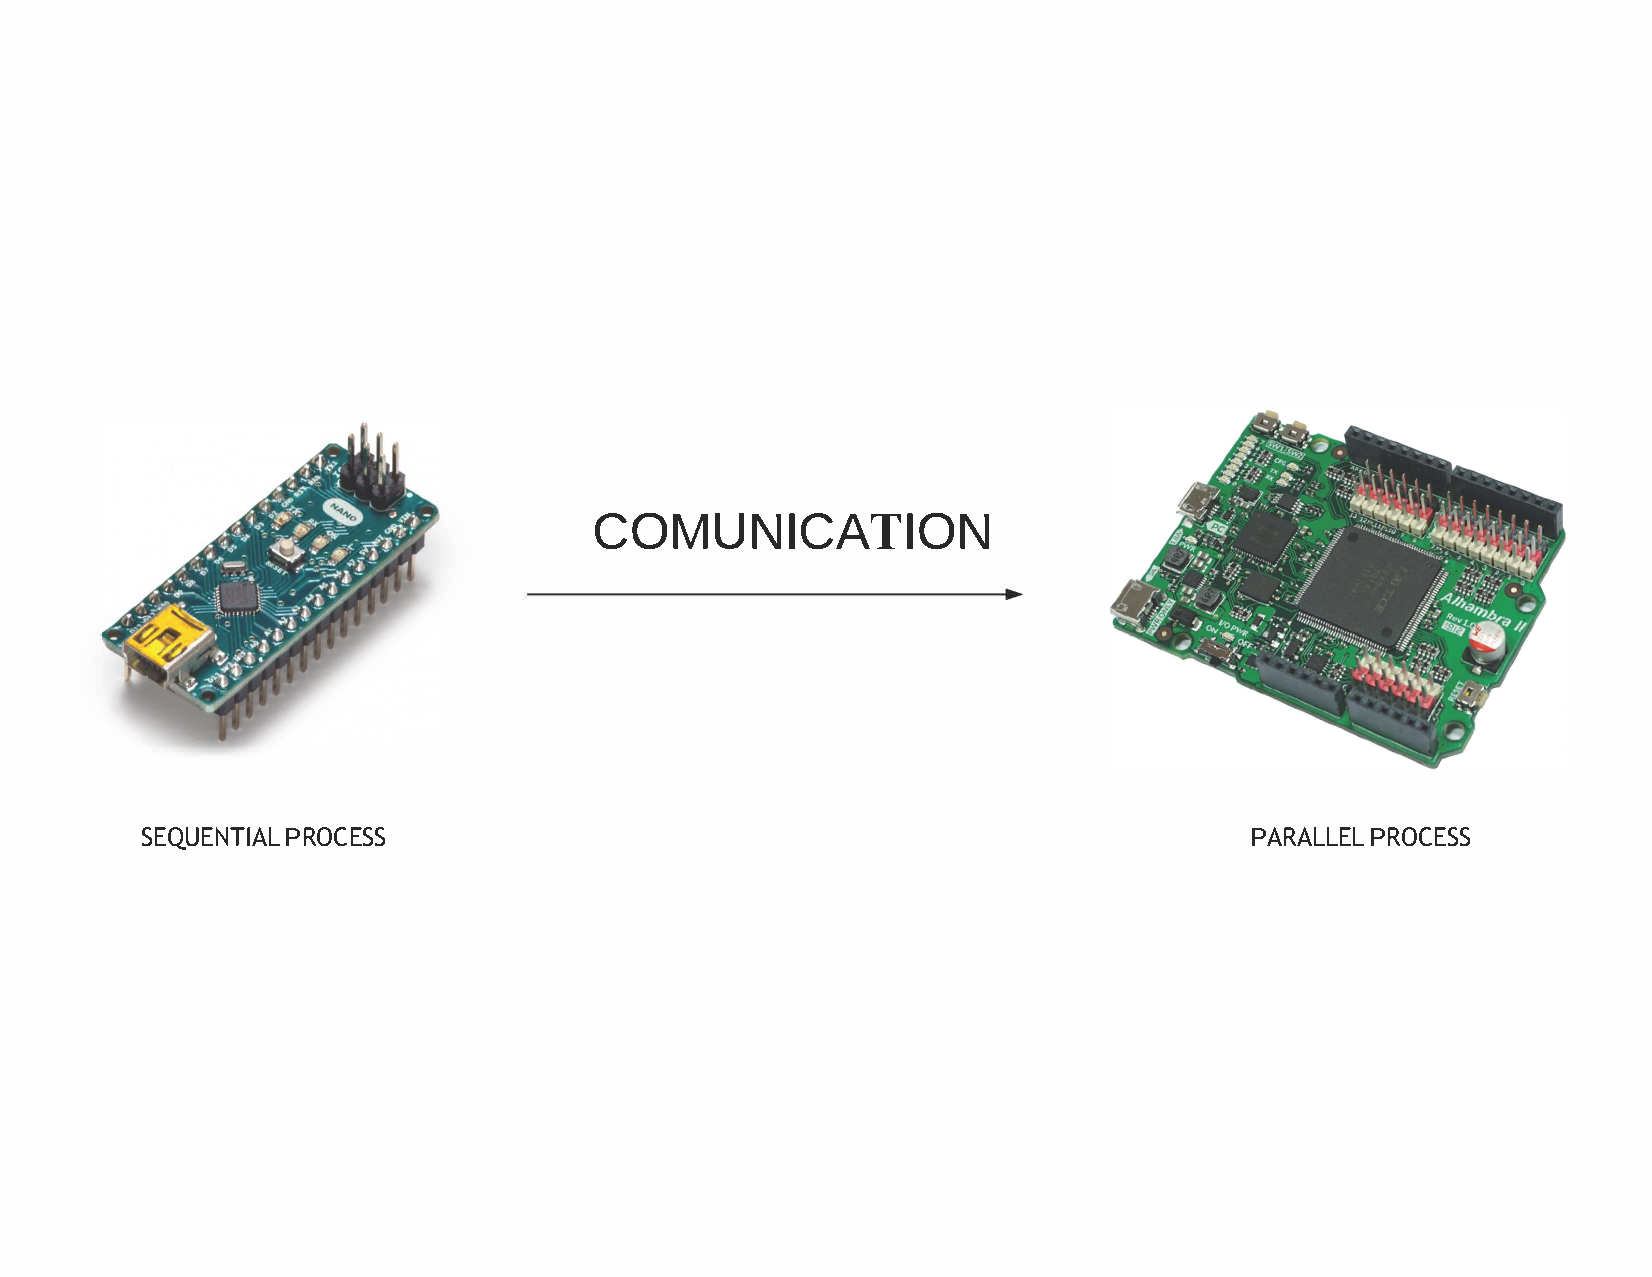
\includegraphics[trim = 0mm 40mm 0mm 20mm, clip,scale=0.4]{imagenes/Balancing_robot/coexistencia1.pdf}
	\caption{Separación de procesos micro-FPGA.}
	\label{fig:coexistencia1}
\end{figure}

En este caso, la comunicación será solo uni-direccional, el micro-controlador enviará información a la FPGA sobre el ángulo actual del objeto en cuestión con el objetivo de que la FPGA analice y actué a partir de ese ángulo.\newline

Se hace una separación por tanto de dos partes de la comunicación, desde el punto de vista del micro-controlador, y desde el punto de vista de la FPGA. Ambos serán explicados más específicamente en la implementación del sistema pero un diagrama de bloques de alto nivel se representan en las figuras \ref{fig:extraccion_angulo} y \ref{fig:arduino_interfacefluid} respectivamente. 

\subsubsection{Desde el punto de vista del micro-controlador:}

\begin{figure}[H]
	\center
	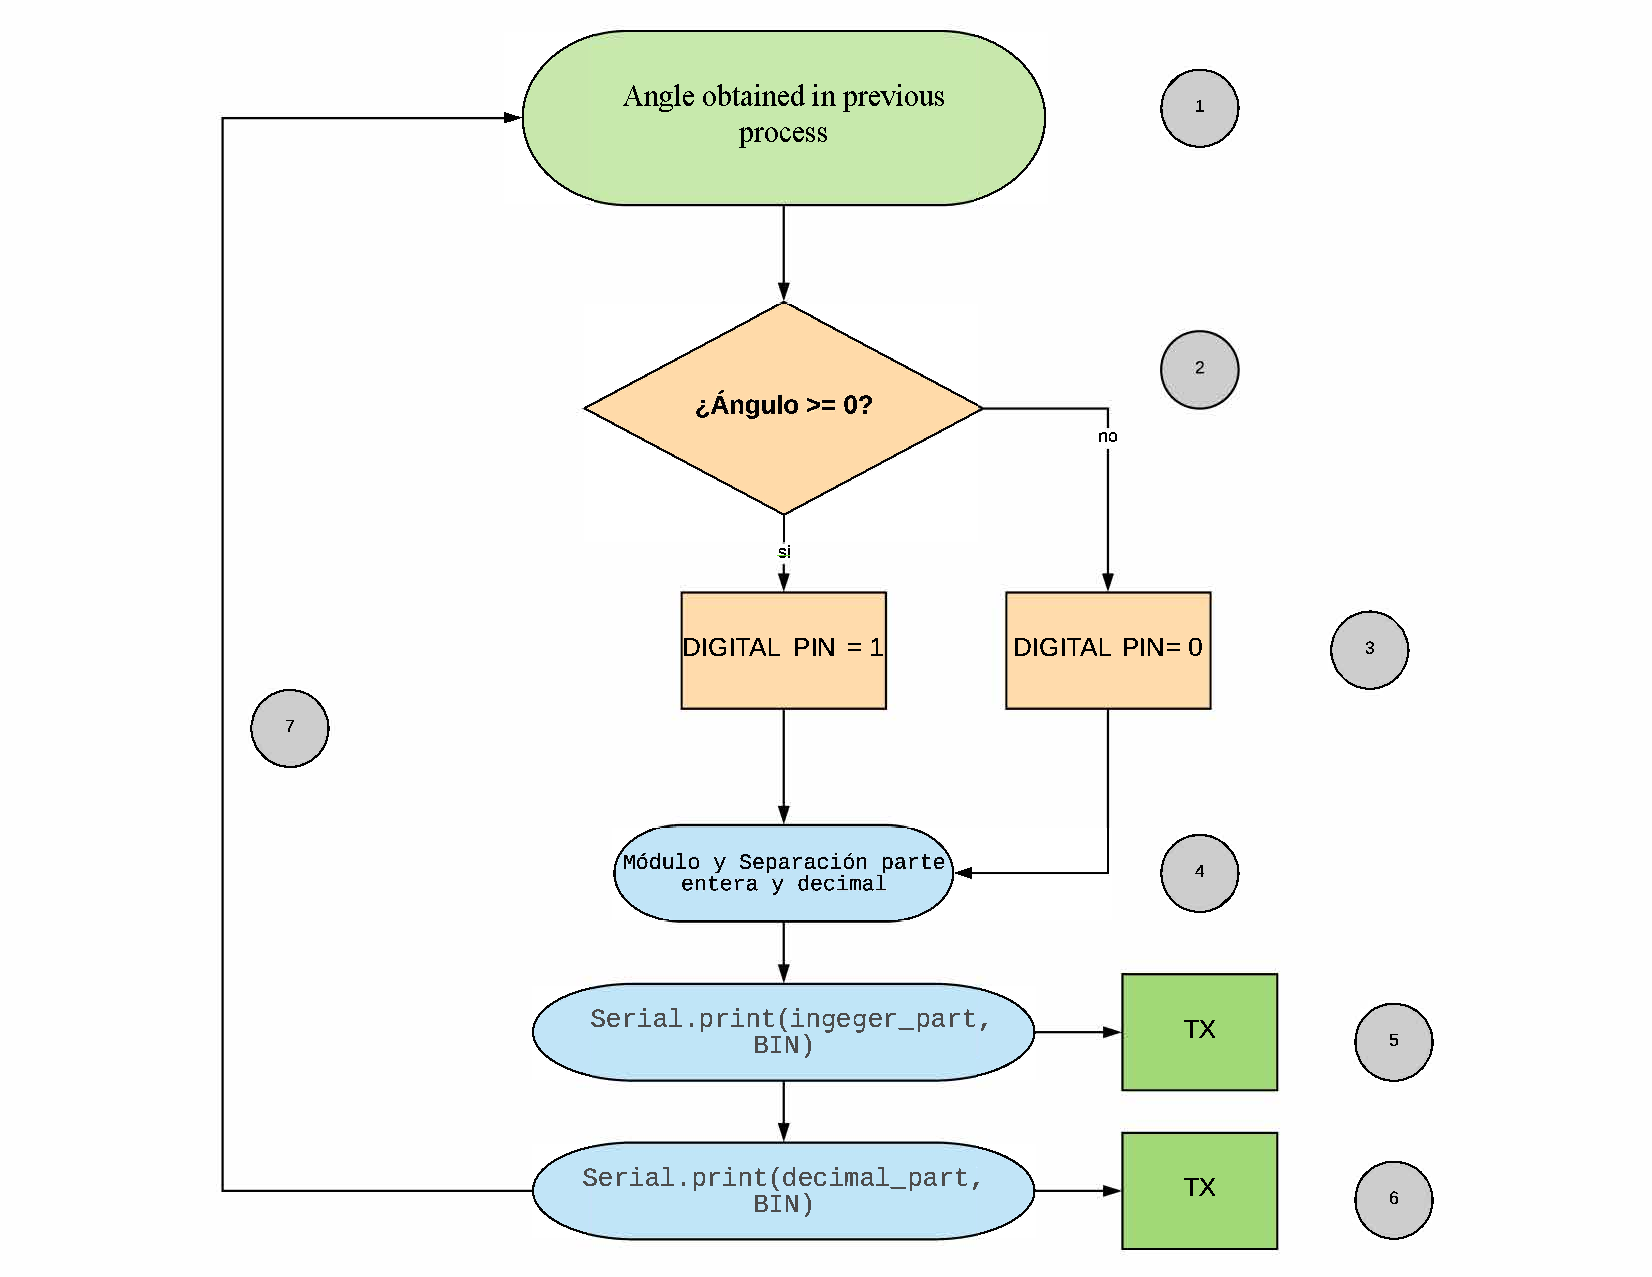
\includegraphics[trim = 0mm 0mm 0mm 0mm, clip,scale=0.7]{imagenes/Balancing_robot/extraccion_angulo.pdf}
	\caption{Envío de ángulo usando el puerto serie.}
	\label{fig:extraccion_angulo}
\end{figure}

\subsubsection{Desde el punto de vista de la FPGA:}
\begin{center}
	\begin{figure}[H]
		\center
		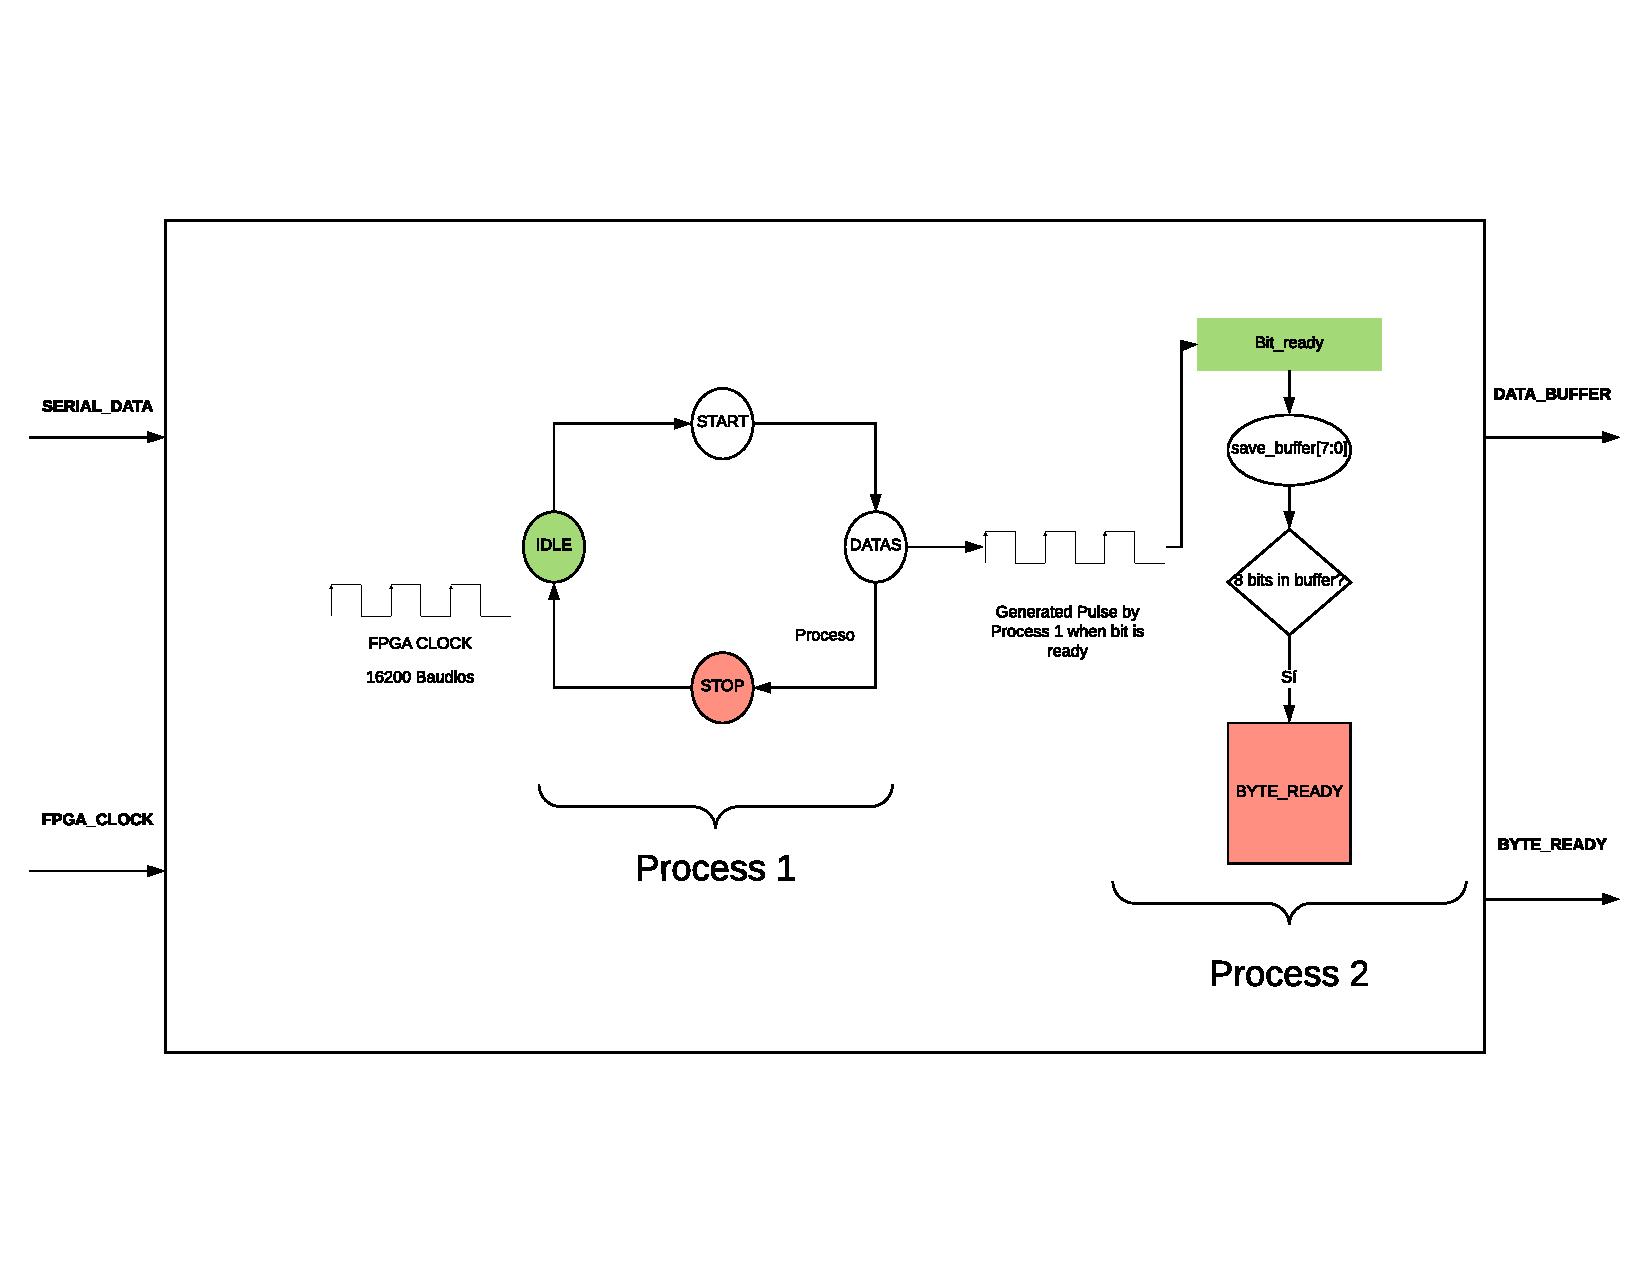
\includegraphics[trim = 0mm 0mm 0mm 10mm, clip,scale=0.9, angle=90]{imagenes/Balancing_robot/arduino_interfacefluid.pdf}
		%\caption{Diagrama de flujo de la interfaz para Arduino.}
		\label{fig:arduino_interfacefluid}
	\end{figure}
\end{center}

El aspecto en IceStudio del módulo anterior (\ref{fig:arduino_interfacefluid}) se muestra en la imagen \ref{fig:arduino_interface}. Si se aprecia, sus entradas y salidas tienen mucho que ver con las características requeridas para la lectura correcta de un byte.

\begin{figure}[H]
	\center
	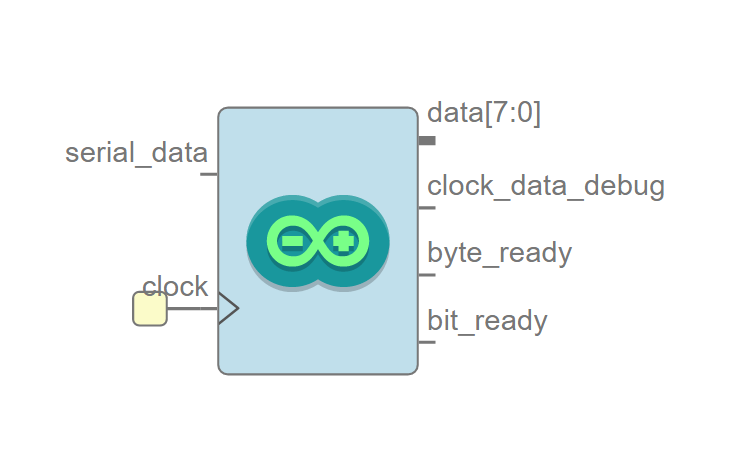
\includegraphics[scale=0.6]{imagenes/Balancing_robot/arduino_interface.PNG}
	\caption{Apariencia del módulo interfaz de Arduino Nano en IceStudio.}
	\label{fig:arduino_interface}
\end{figure}

Se hace necesario un módulo adicional que ordene tanto la parte entera como la parte decimal del ángulo correspondiente y que no provoque errores en la obtención del ángulo (figura \ref{fig:arrange_arduino}). 

\begin{figure}[H]
	\center
	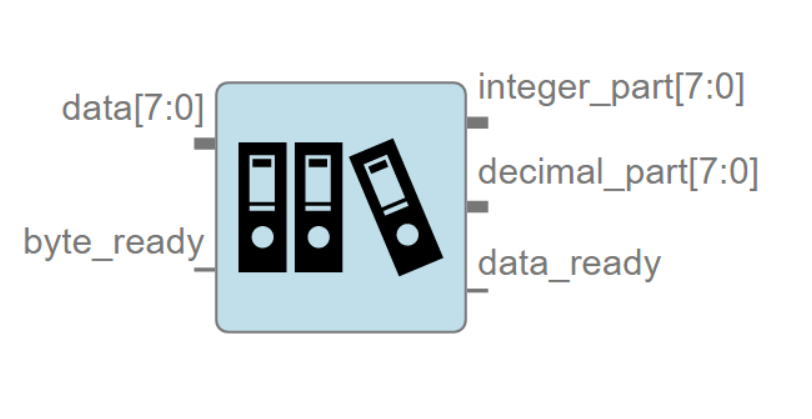
\includegraphics[scale=0.4]{imagenes/Balancing_robot/arrange_arduino.PNG}
	\caption{Módulo para ordenar datos provenientes de Arduino.}
	\label{fig:arrange_arduino}
\end{figure}


El sistema final de comunicación entre Arduino y IceZum Alhambra desde el punto de vista de la FPGA se representa en la figura \ref{fig:arduino_arrange}.

\begin{figure}[H]
	\center
	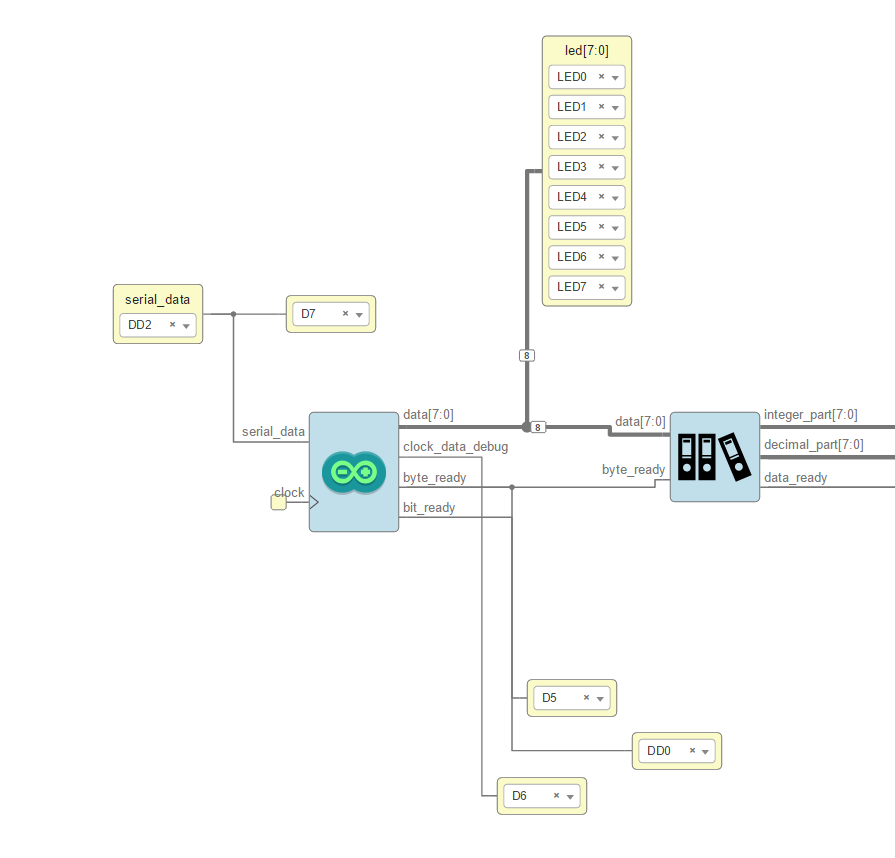
\includegraphics[scale=0.6]{imagenes/Balancing_robot/arduino_arrange.PNG}
	\caption{Solución final en FPGA de la comunicación entre Arduino y IceZum Alhambra.}
	\label{fig:arduino_arrange}
\end{figure}






Una integración entre un micro-controlador y FPGA permite diferenciar tareas secuenciales y paralelas, asignando cada proceso o bien al micro-controlador si necesariamente tiene que ser secuencial o bien a la FPGA si el proceso puede se paralelizado y obtener con ello algunas ventajas. \newline

Hay varias opciones para hacer una integración Micro-Controlador--FPGA:

\begin{itemize}
	\item Emular el comportamiento de un micro-controlador en una FPGA.
	\item Coexistencia física de una FPGA y micro-controlador creando una comunicación entre cada una de ellas.
\end{itemize}
En este proyecto se ha elegido la segunda como opción por no contar con los recursos suficientes para llevar a cabo la primera, a pesar de que esta sería la mas adecuada en cuanto ahorro de recursos y facilidad de uso. \newline

Así se hace necesario una comunicación micro-controlador/FPGA. Existen dos tipos de comunicación posibles para este propósito: 
\begin{itemize}
	\item Comunicación serie: Es una comunicación secuencial, se envían los bits uno a uno, secuencialmente y haciendo uso solo de un bus de datos.
	\item Comunicación en paralelo: Todos los bits de cada símbolo se envían a la vez.
\end{itemize} 

Para hacer uso de la comunicación en paralelo se necesitan tantos canales como bits tenga la información a transmitir (si se quiere enviar un byte se debería hacer uso de un total de 8 canales, correspondientes a cada bit). En este caso habría que utilizar 8 pines de la FPGA para poder llevar a cabo este tipo de transmisión. Por ello, y a pesar de que la comunicación paralela es mas rápida que en serie, se elije la primera como opción más conveniente. \newline

El tipo de comunicación serie desarrollada podría asemejarse a un protocolo SPI, aunque sólo tiene capacidad para datos en una dirección. El esquemático de esta comunicación desarrollada es el expuesto en la figura \ref{fig:coexistencia2}.

\begin{figure}[H]
	\center
	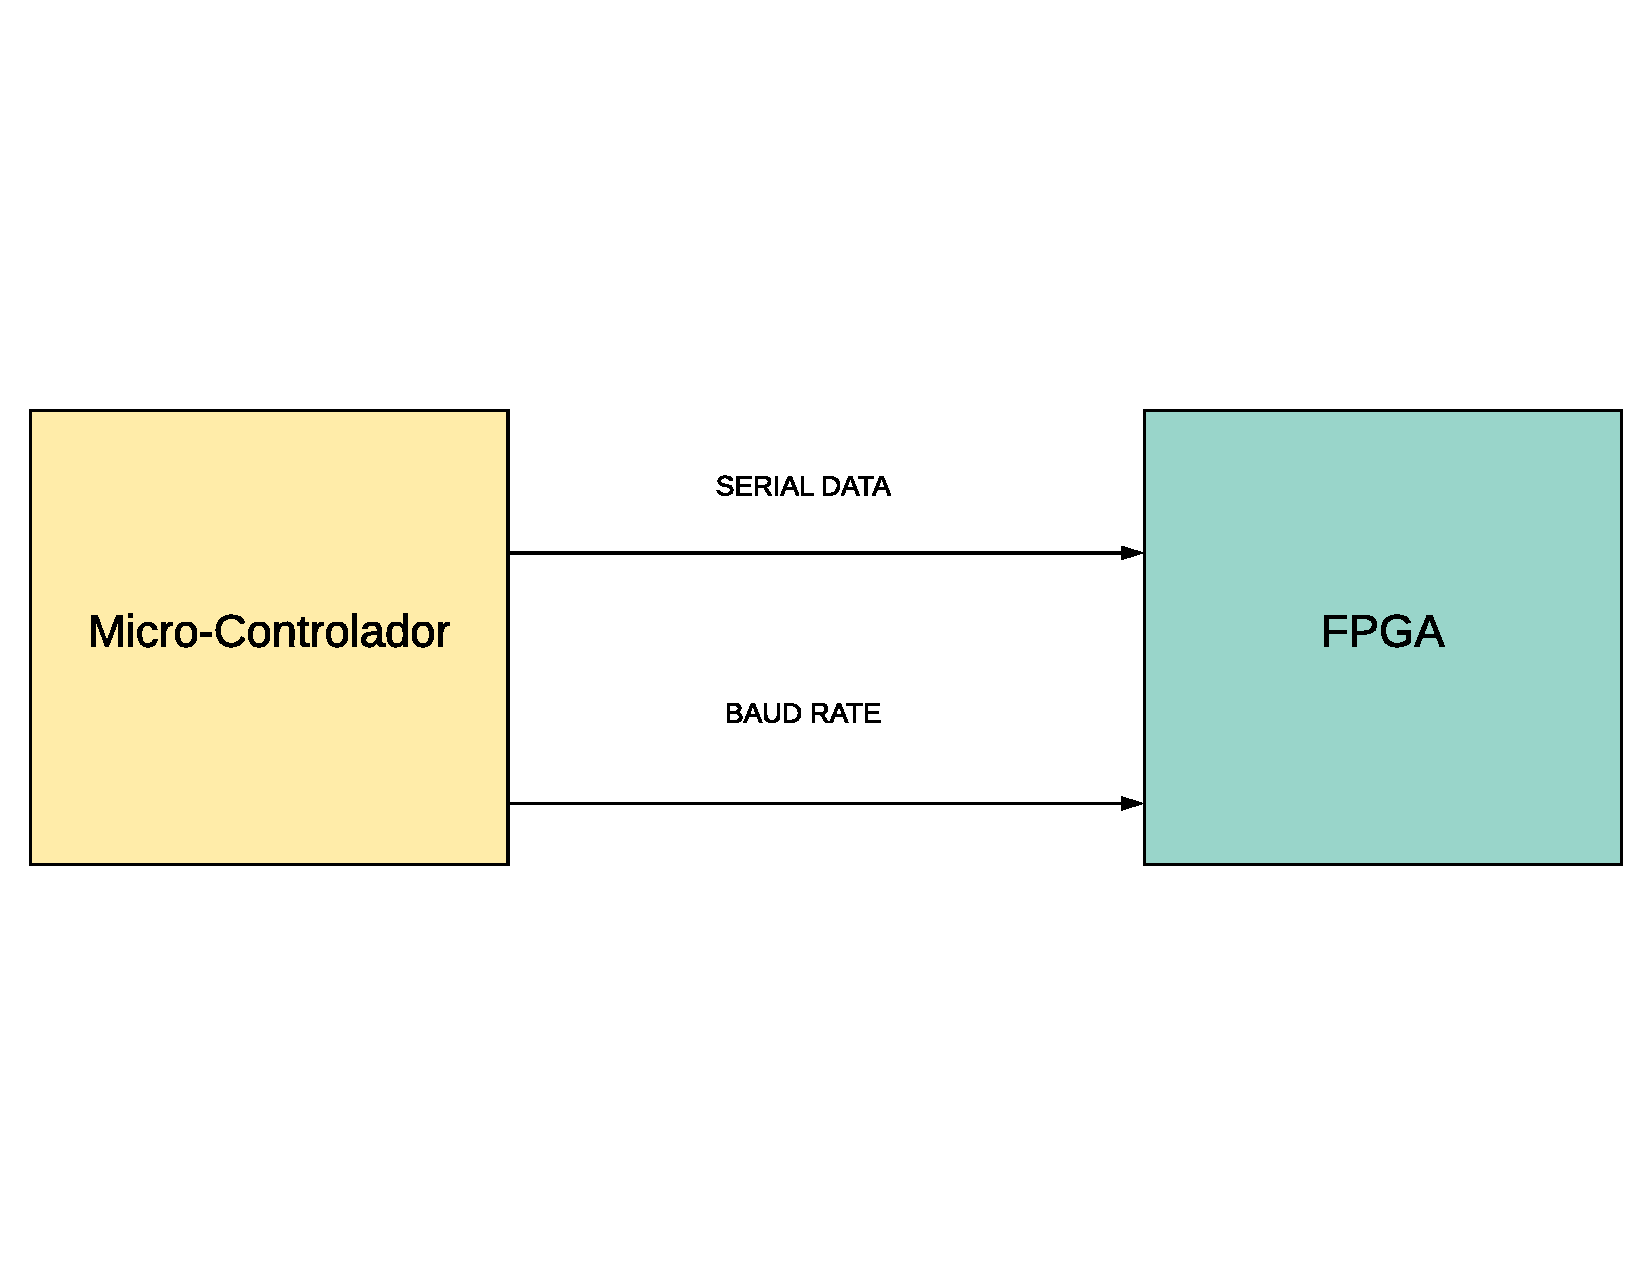
\includegraphics[trim = 0mm 40mm 0mm 20mm, clip,scale=0.4]{imagenes/Balancing_robot/coexistencia2.pdf}
	\caption{Pines hardware de coexistencia micro-FPGA.}
	\label{fig:coexistencia2}
\end{figure}
El sistema general cuenta con dos conexiones:
\begin{itemize}
	\item Una línea de datos para el envió de la información.
	\item Una linea de reloj para que la FPGA pueda obtener en todo momento la velocidad de la información.
\end{itemize}

Un posible ejemplo de una comunicación en serie de un byte de datos podría ser el siguiente: 
\textbf{Ejemplo com SPI}


Se introduce a más bajo nivel las dos partes, la comunicación desde el punto de vista del micro-controlador y la comunicación desde el punto de vista de la FPGA. 

\subsubsection{Desde el punto de vista del micro-controlador:}

Para el desarrollo de este sub-capítulo se parte de la base de que el ángulo actual ya ha sido obtenido en el micro-controlador. Así, y para la claridad del lector, un esquemático interno del arduino nano es mostrado en la figura \ref{fig:coexistencia3}. En este apartado y con respecto a la parte del micro-controlador, solo se analiza la parte sombreada.  

\begin{figure}[H]
	\center
	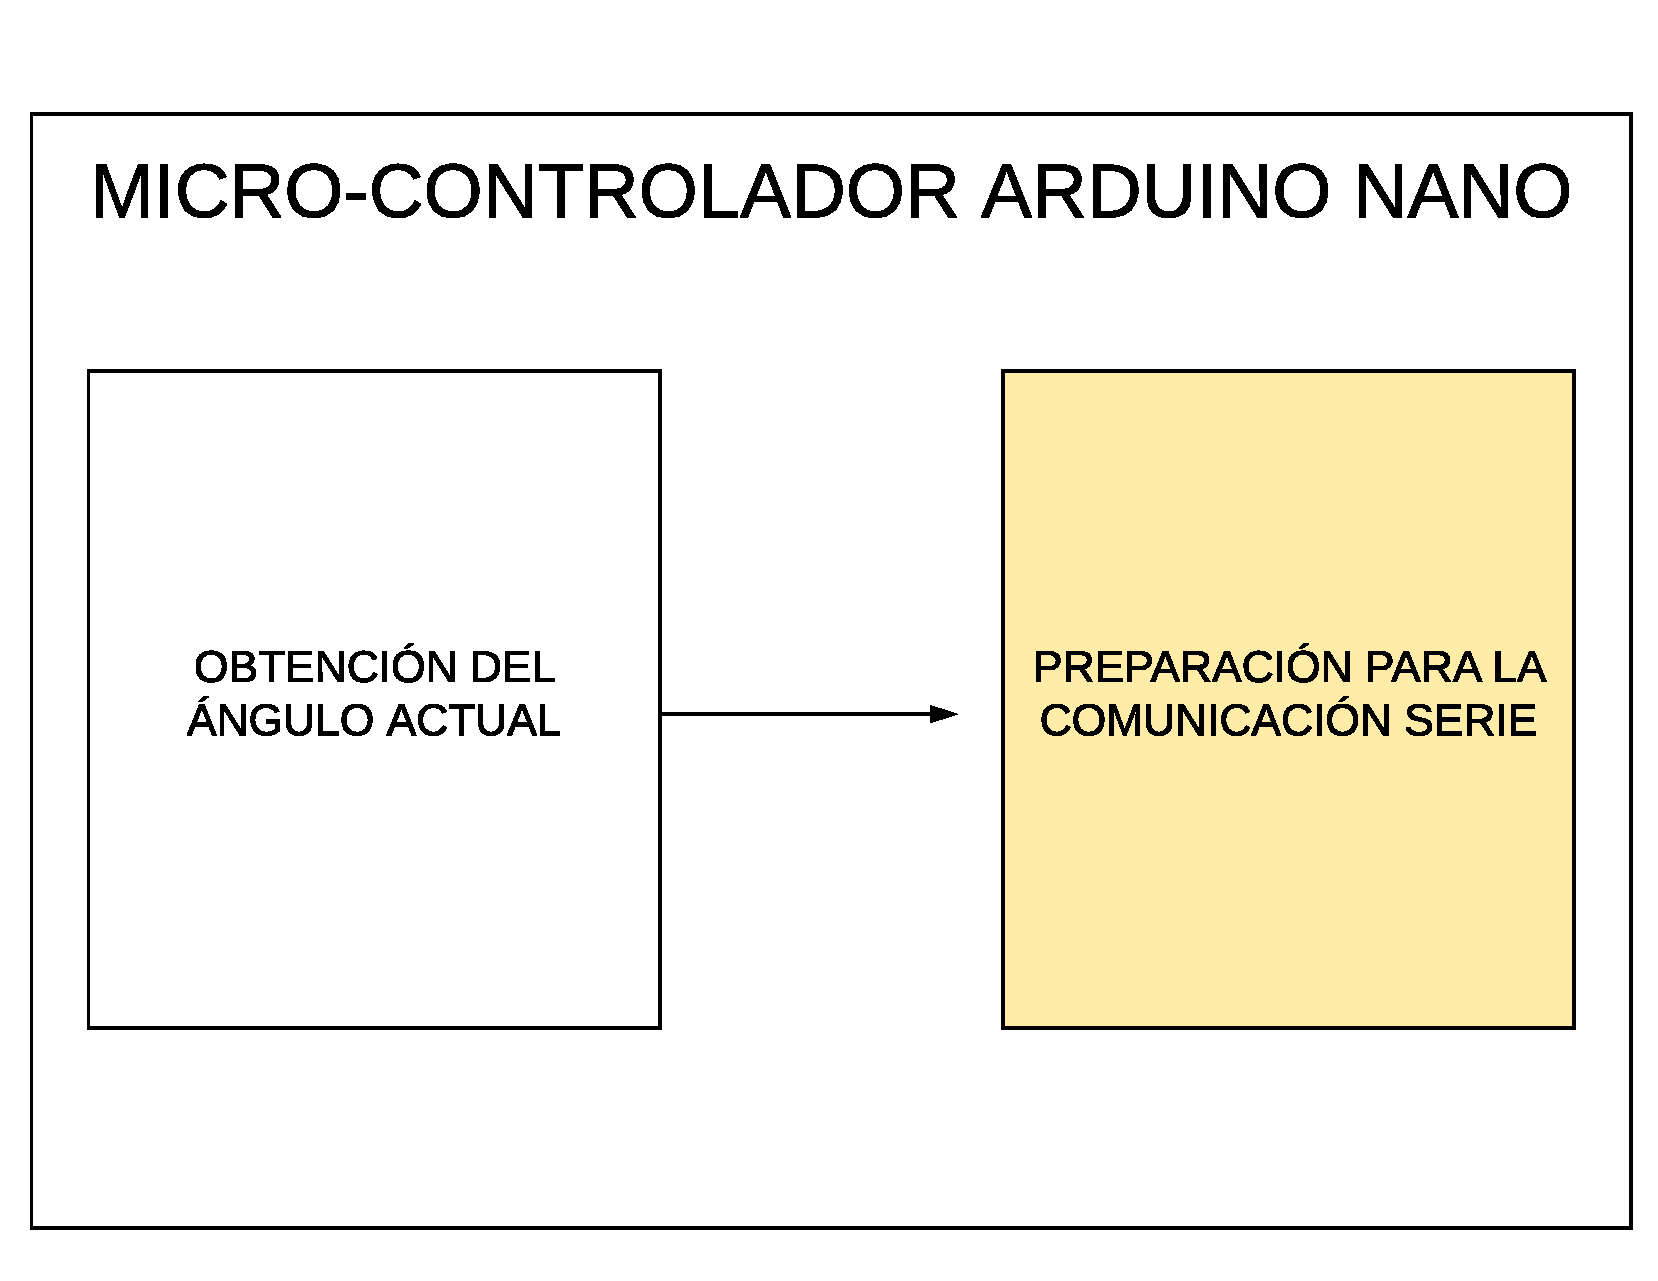
\includegraphics[trim = 0mm 0mm 0mm 0mm, clip,scale=0.3]{imagenes/Balancing_robot/coexistencia3.pdf}
	\caption{Diagrama interno Arduino Nano.}
	\label{fig:coexistencia3}
\end{figure}

El diagrama de flujo sobre el cuál se basa el código en C del micro-controlador se representa en la figura \ref{fig:extraccion_angulo}

A continuación se pasa a explicar los aspectos mas relevantes: 

\begin{itemize}
	\item \textbf{1.-}Se parte de la base de que el ángulo ya ha sido obtenido y es correcto. En la sección \ref{sec:MPU6050} se puede encontrar más información sobre ello.
	\item \textbf{2.-}Una de las partes más importantes para corregir el control del balancín es conocer la inclinación en cada momento para poder corregir esta desviación (figura en la que se ve como se hace esa corrección). Para ello, la FPGA debe conocer si el ángulo es positivo o negativo. Este aspecto no formará parte del propio protocolo de comunicación como se verá a continuación.
	\item \textbf{3.-}Se utiliza un solo pin del micro-controlador el cuál cambiará su valor a 1 o 0 dependiendo del signo del ángulo en cada momento. Así, la FPGA sólo tendrá que leer esta información cuando le sea necesario.
	\item \textbf{4.-}Para un correcto entendimiento por parte de la FPGA es necesario enviar el ángulo representado en bytes y no en código ASCII. Es por ello que para ese envío de utilizará el comando "Serial.print(ángulo)". Esta función de arduino envía por el puerto serie la representación en bytes del ángulo en cuestión.\newline
	Si se intenta enviar todo el ángulo también se enviarán tanto el símbolo como el código ASCII de la coma y esto es un aspecto que no interesa tener en cuenta en lo que al procesamiento sobre la FPGA se refiere. Para corregirlo primero se hace el módulo del ángulo (no se necesita el signo porque ya hay un pin destinado para ello) y posteriormente de hace una separación entre la parte entera y la parte decimal para poder eliminar el carácter "comma". 
	
	\item \textbf{5.-}Se envía por el puerto serie el byte correspondiente a la parte entera. 
	\item \textbf{6.-}Se envía por el puerto serie el byte correspondiente a la parte decimal. 
	\item \textbf{7.-}Es un proceso cíclico que se irá reproduciendo cada X segundos, esto es, el ángulo podrá corregirse cada X segundos. 
\end{itemize}
Un ejemplo real del envío del un ángulo con su correspondiente signo es mostrado en la figura \ref{label}

\subsubsection{Desde el punto de vista de la FPGA:} \newline

Por un PIN de entrada a la FPGA le estarán continuamente entrando datos provenientes del pin de transmisión y para que se puede hacer una lectura correcta del byte es necesario conocer: 

\begin{itemize}
	\item Cuando comienza una transmisión de un byte.
	\item Cuando termina una transmisión de un byte.
	\item Cuando un bit puede ser capturado. 
	\item Se vayan almacenando en un buffer los bits necesarios hasta que el byte este completo.
\end{itemize}

Para poder implementar en la FPGA un módulo intermedio con las anteriores carácteristicas  (figura \ref{fig:arduino_interface})es necesario conocer de antemano la velocidad de la transmisión por parte del micro-controlador, la cuál se ha fijado en 16200 baudios. \newline

Se detallan las diferentes entradas y salidas del módulo anterior: 

\begin{itemize}
	\item data[7:0]: Consiste en un buffer en el cuál se van almacenando los bits cuando es necesario hasta tener el byte. Es importante que el módulo siguiente conozca cuando el byte esta preparado para su captura.
	\item clock\_data\_debug: La utilización de esta salida es sólo para depuración.
	\item byte\_ready: Un flag de reloj cambiará su valor cuando un byte este listo para ser capturado. Como se ha visto en anteriores desarrollos, este byte será o bien la parte entera o bien la parte decimal.
	\item bit\_ready: La utilización de esta salida de solo para depuracion.
\end{itemize} 

La implementación en IceStudio del comportamiento anterior está implementada mediante dos máquinas estados con sus correspondientes listas de sensibilidad, y el diagrama de flujo se representa en la figura \ref{fig:arduino_interfacefluid}. Se hace uso de dos procesos bien diferenciados:

\textbf{Proceso 1:} Este proceso solo dota al sistema siguiente del momento exacto en el cual puede capturar un bit y guardarlo en el buffer, para ello, debe conocer la velocidad de la transmisión comentada anteriormente. Los estados serán los siguientes: 

\begin{itemize}
	\item IDLE: El proceso se mantiene en este estado hasta que se inicie la transmisión, que pasará al siguiente estado (START).
	\item START: Como se ha desarrollado en la seccion \ref{label} el protocolo de transmision serie comienza con una condicion de start, este estado permitirá reconocer cuando acaba esta condicion para poder empezar a guardar bits en el buffer. 
	\item DATAS: Como ya se conoce la velocidad de transmision y se ha reconocido la condicion de START en el estado anterior, en este estado un flag cambiará su valor cuando el bit este preparado para ser guardado en el buffer, de lo cuál se encargará el proceso 2.
	\item STOP: Además de una condición de START, el protocolo de transmisión en serie usado en Arduino tiene un condición de STOP. Este estado permite reconocer el tiempo que tarda Arduino en llevar a cabo esta ultima condicion, después, volverá al primer estado hasta que empiece una nueva transacción.
\end{itemize}

\textbf{Proceso 2:} El proceso 2 está activado por el proceso 1. Cuando el proceso 1 determine que un bit está disponible en el bus para ser capturado, pondrá en alta un flag de reloj, iniciando el proceso 1 mediante una lista de sensibilidad. El diagrama de flujo podría ser:

\begin{itemize}
	\item Esperar hasta que se active al lista de sensibilidad, eso indicará que un bit podrá ser capturado.
	\item Los bits se irán guardando en un buffer que formará un byte, el cuál representa la parte entera o decimal del ángulo en ese momento.
	\item Cuando el byte este preparado para ser capturado por los consecutivos módulos un canal se pondrá en alta, estando disponibles como salidas tanto el buffer con 8 los bits y este canal de "byte\_ready".
\end{itemize}

En este punto la FPGA es capaz de diferenciar cuando puede capturar un byte (BYTE\_READY) y de donde tiene que capturar el bus de datos (DATA\_BUFFER). No obstante un aspecto que no forma parte de la comunicación en sí es importante de analizar si se quiere conseguir un correcto funcionamiento. Esto es, si se ha dicho anteriormente que el micro-controlador envía continuamente la parte entera y decimal del ángulo, si no se hace una buena interpretación de estos datos, es posible que un ángulo sobre la FPGA este formado por una parte decimal de un angulo n y la parte entera del ángulo n+1. \newline

Para ello se crea un módulo en IceStudio que sea capaz de ordenar estos valores. El aspecto de este módulo en IceStudio se muestra en la figura \ref{fig:arrange_arduino}

Como entradas:

\begin{itemize}
	\item data[7:0] : Es el buffer de salida del modulo anterior donde se van acumulando los bits capturados hasta conseguir el byte.
	\item byte\_ready : Flag de reloj que se activa cuando el byte este disponible para ser capturado.
\end{itemize}

Es importante tener en cuenta que el dato estará disponible siempre y cuando este disponible tanto la parte entera como la parte decimal del ángulo en cuestión. Así, como salidas se encuentran:

\begin{itemize}
	\item integer\_part[7:0] : byte que representa la parte entera del ángulo.
	\item decimal\_part[7:0] : byte que representa la parte decimal del ángulo.
	\item data\_ready : flag de reloj que se activa cuando el dato (parte decimal y parte entera) este preparado para ser capturado.	
\end{itemize}

Como se ha profundizado anteriormente, el diagrama de flujo que explica el código en Verilog que implementa el anterior comportamiento se representa en la figura \ref{fig:arrange_angle} y será comentado mas adelante.

\begin{figure}[H]
	\center
	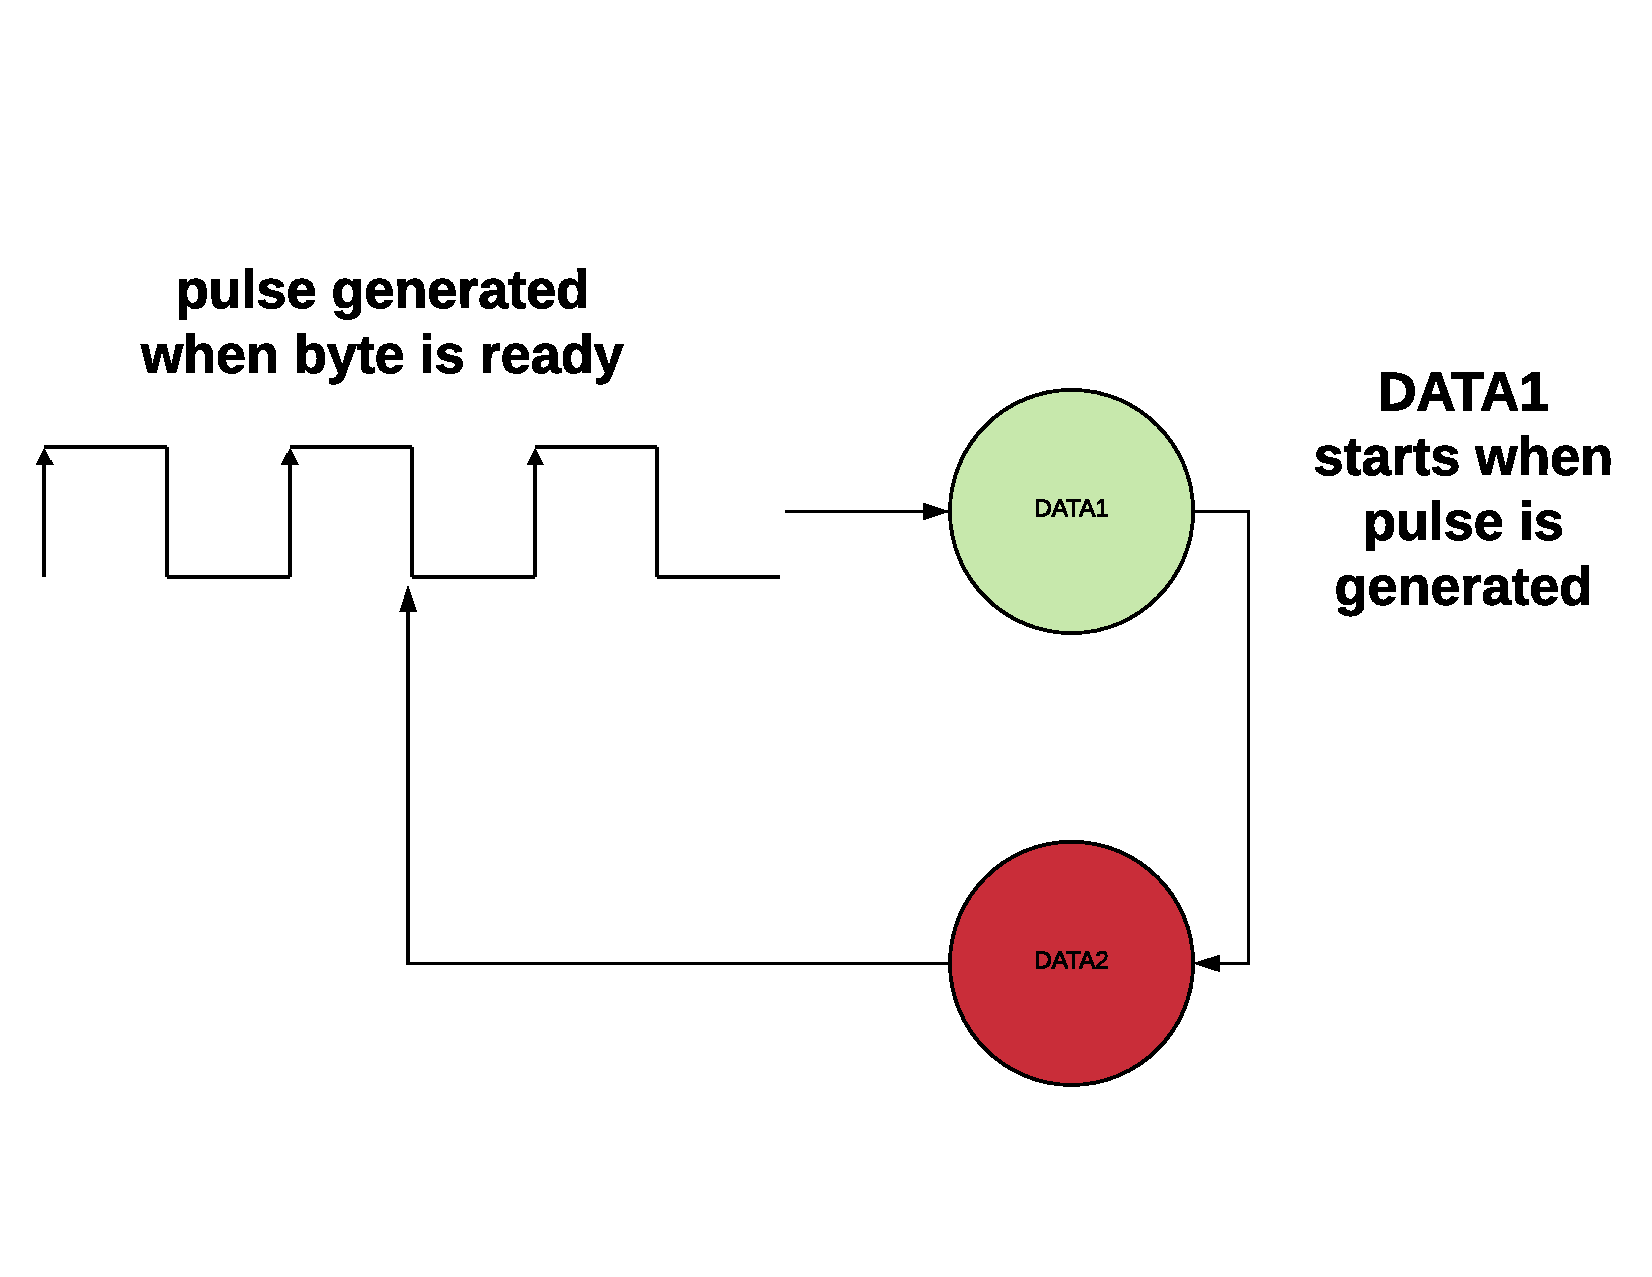
\includegraphics[scale=0.5]{imagenes/Balancing_robot/arrange_angle.pdf}
	\caption{Diagrama de flujo modulo ordenación de bytes.}
	\label{fig:arrange_angle}
\end{figure}



En este caso es un proceso con una lista de sensibilidad que cuenta como señal sensible el bus de "byte\_ready", y que es salida del modulo anterior. \newline

Cada vez que se active el flag que indica que un byte está listo para ser capturado comienza una máquina de estados cíclica que cuenta con los dos siguientes estados:

\begin{itemize}
	 \item DATA1: Es el primer dato a ser capturado y corresponde con la parte entera del primer ángulo. La segunda vez que se active el flag de "byte\_ready" corresponderá a la parte decimal del primer ángulo, y por lo tanto pasará al siguiente estado DATA2.
	 \item DATA2: En ese estado no sólo se captura la parte decimal del ángulo en cuestión sino que además se activa un nuevo flag el cuál indica que el dato completo (ángulo) esta listo para ser capturado. 
\end{itemize}

Así, el módulo tendrá como salidas el buffer de la parte entera, el buffer de la parte decimal, y un bus que avisará a los sucesivos módulos de cuándo el dato completo está preparado para ser capturado. De esta forma se ha evitado el problema explicado anteriormente de la no ordenación en los datos llegados del micro-controlador.  \newline

Se da por finalizado el protocolo de comunicación Arduino-FPGA y se brindan las herramientas necesarias para que los sucesivos procesos y módulos puedan conocer el ángulo en cada momento representado por su parte entera (8 bits), parte decimal (8 bits) y un pin que indicará el valor del signo (positivo o negativo).




\subsection{Control PID}
\subsection{Integración control PID en IceZum Alhambra}
Como ha sido explicado en la sección \ref{sec:PID}, un controlador PID puede ser utilizado de manera sencilla para controlar la estabilidad del sistema. \newline
El aspecto en IceStudio de estos bloques de control se ilustra en las figuras \ref{fig:Pcontrol} y \ref{fig:Dcontrol}.

\begin{figure}[H]
	\center
	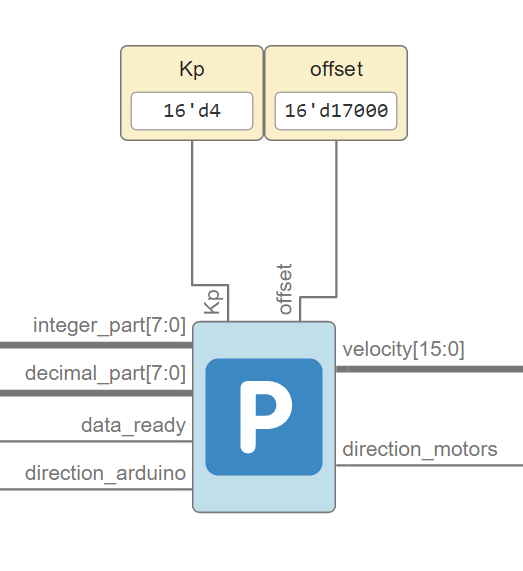
\includegraphics[scale=0.5]{imagenes/Balancing_robot/Pcontrol}
	\caption{Aspecto en IceStudio del módulo de control P.}
	\label{fig:Pcontrol}
\end{figure}

\begin{figure}[H]
	\center
	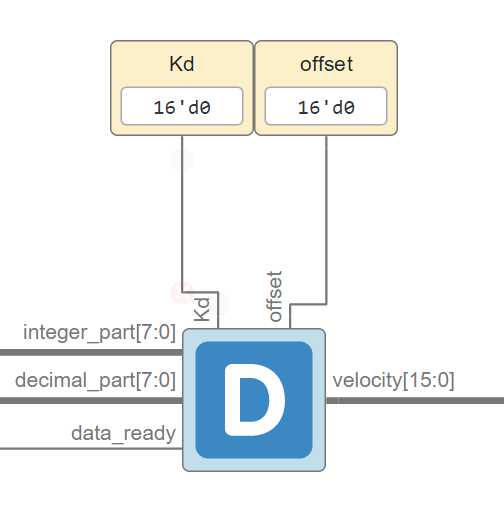
\includegraphics[scale=0.5]{imagenes/Balancing_robot/Dcontrol}
	\caption{Aspecto en IceStudio del módulo de control D.}
	\label{fig:Dcontrol}
\end{figure}

Referido al sistema de realimentación por lazo cerrado analizado en la sección \ref{sec:PID}, es importante mostrar el resultado final del aspecto del presente proyecto en IceStudio, haciendo una comparativa directa entre éste (figura \ref{fig:finalIceStudio} ) y la figura \ref{fig:PID}.
\newpage
\begin{figure}[H]
	\center
	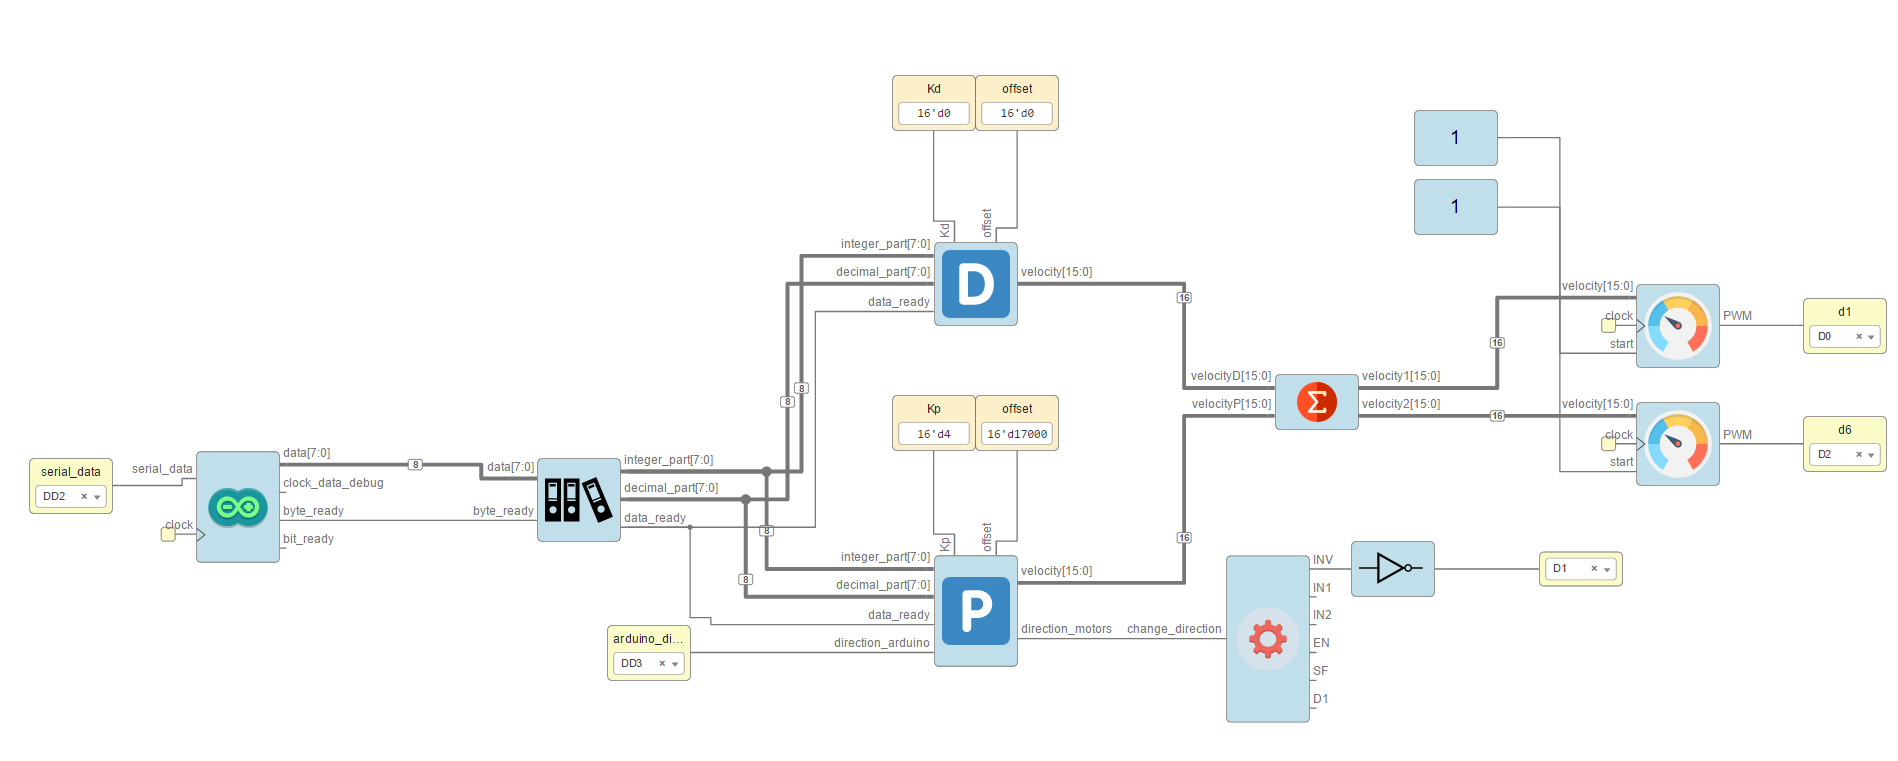
\includegraphics[scale=0.6, angle=90]{imagenes/Balancing_robot/finalIceStudio}
	\caption{Aspecto final en IceStudio del Balancing-Robot.}
	\label{fig:finalIceStudio}
\end{figure}

\subsection{Driver motores DC} \label{sec:driver_motores}

\subsection{Controlador de motores}
Tener un modulo con la capacidad para generar PWM soluciona muchos problemas posteriores a la vez que mejora la visibilidad del código en el sistema final. Como se observa en las características de los motores, gran parte de ellos están comandados por una señal PWM que si bien es cierto, depende del motor en cuestión. \newline
La modulación por ancho de pulsos o PWM (Pulse Width Modulation) es una técnica en la que se modifica el ciclo de trabajo de una señal periódica (en nuestro caso cuadrada) que se usa para transmitir información a traves de un canal de comunicación o para controlar la cantidad de energía que se envía a una carga. Un ejemplo de una señal PWM cuadrada es la mostrada en la figura tal 

\textbf{figura PWM}

Aplicando esta señal, por ejemplo, a un motor DC clásico se varia la cantidad de energía que se aplica a la carga, el motor en este caso. Sencillamente funciona como un interruptor en el cuál un nivel lógico alto es abierto y un nivel bajo cerrado. Si se consigue variar el tiempo el cuál al motor le esta llegando carga y el tiempo en el cuál no le llega corriente, se puede controlar su velocidad. \newline

Así, las características de una señal PWM son: 
\begin{itemize}
	\item D = ciclo de trabajo.
	\item $\theta$
	\item T = periodo de la función
\end{itemize}


El driver del motor utilizado para el control de los motores DC (MC33926 []), necesita una serie de configuraciones para poder trabajar acorde a nuestras necesidades. Estas configuraciones se detallan en la sección \ref{sec:driver_motores}. El diagrama final de entradas y salidas así como las conexiones necesarias se detallan en el esquemático de la figura \ref{fig:extraccion_angulo}.


\begin{figure}[H]
	\center
	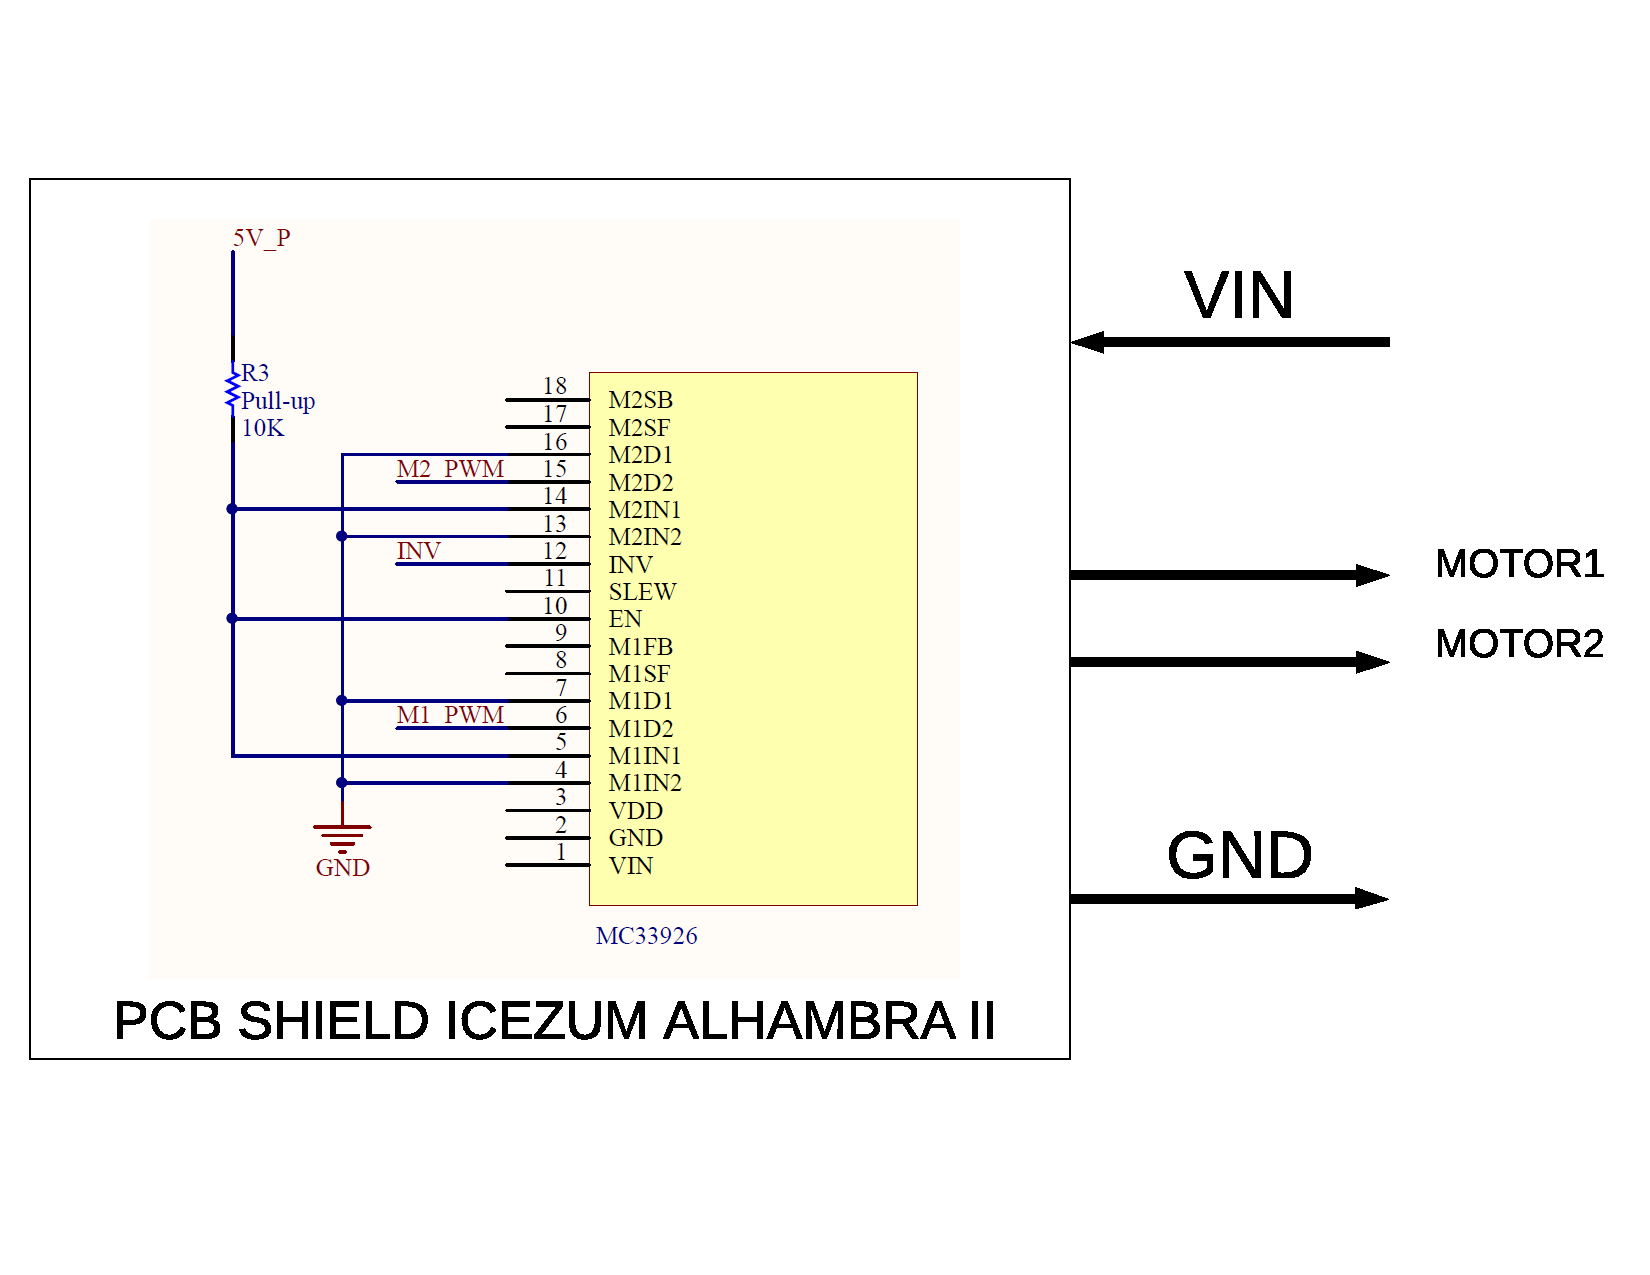
\includegraphics[trim = 0mm 3cm 0mm 2cm, clip,scale=0.6]{imagenes/Balancing_robot/driver_motor.pdf}
	\caption{Envío de ángulo usando el puerto serie.}
	\label{fig:extraccion_angulo}
\end{figure}




\subsubsection{Control PWM}

Los velocidad de los motores se controlan mediante un generador de PWM el cuál tiene el aspecto de la figura \ref{fig:pwm_module} en IceStudio. 

\begin{figure}[H]
	\center
	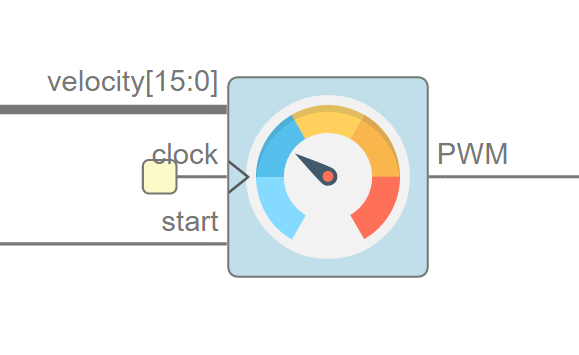
\includegraphics[scale=0.5]{imagenes/Balancing_robot/PWM_module.PNG}
	\caption{Aspecto en IceStudio del generador de señal PWM.}
	\label{fig:pwm_module}
\end{figure}

El diagrama de bloques de su funcionamiento se expone en la figura \ref{fig:pwm_control} tal y se profundizará en su implementación:

\begin{figure}[H]
	\center
	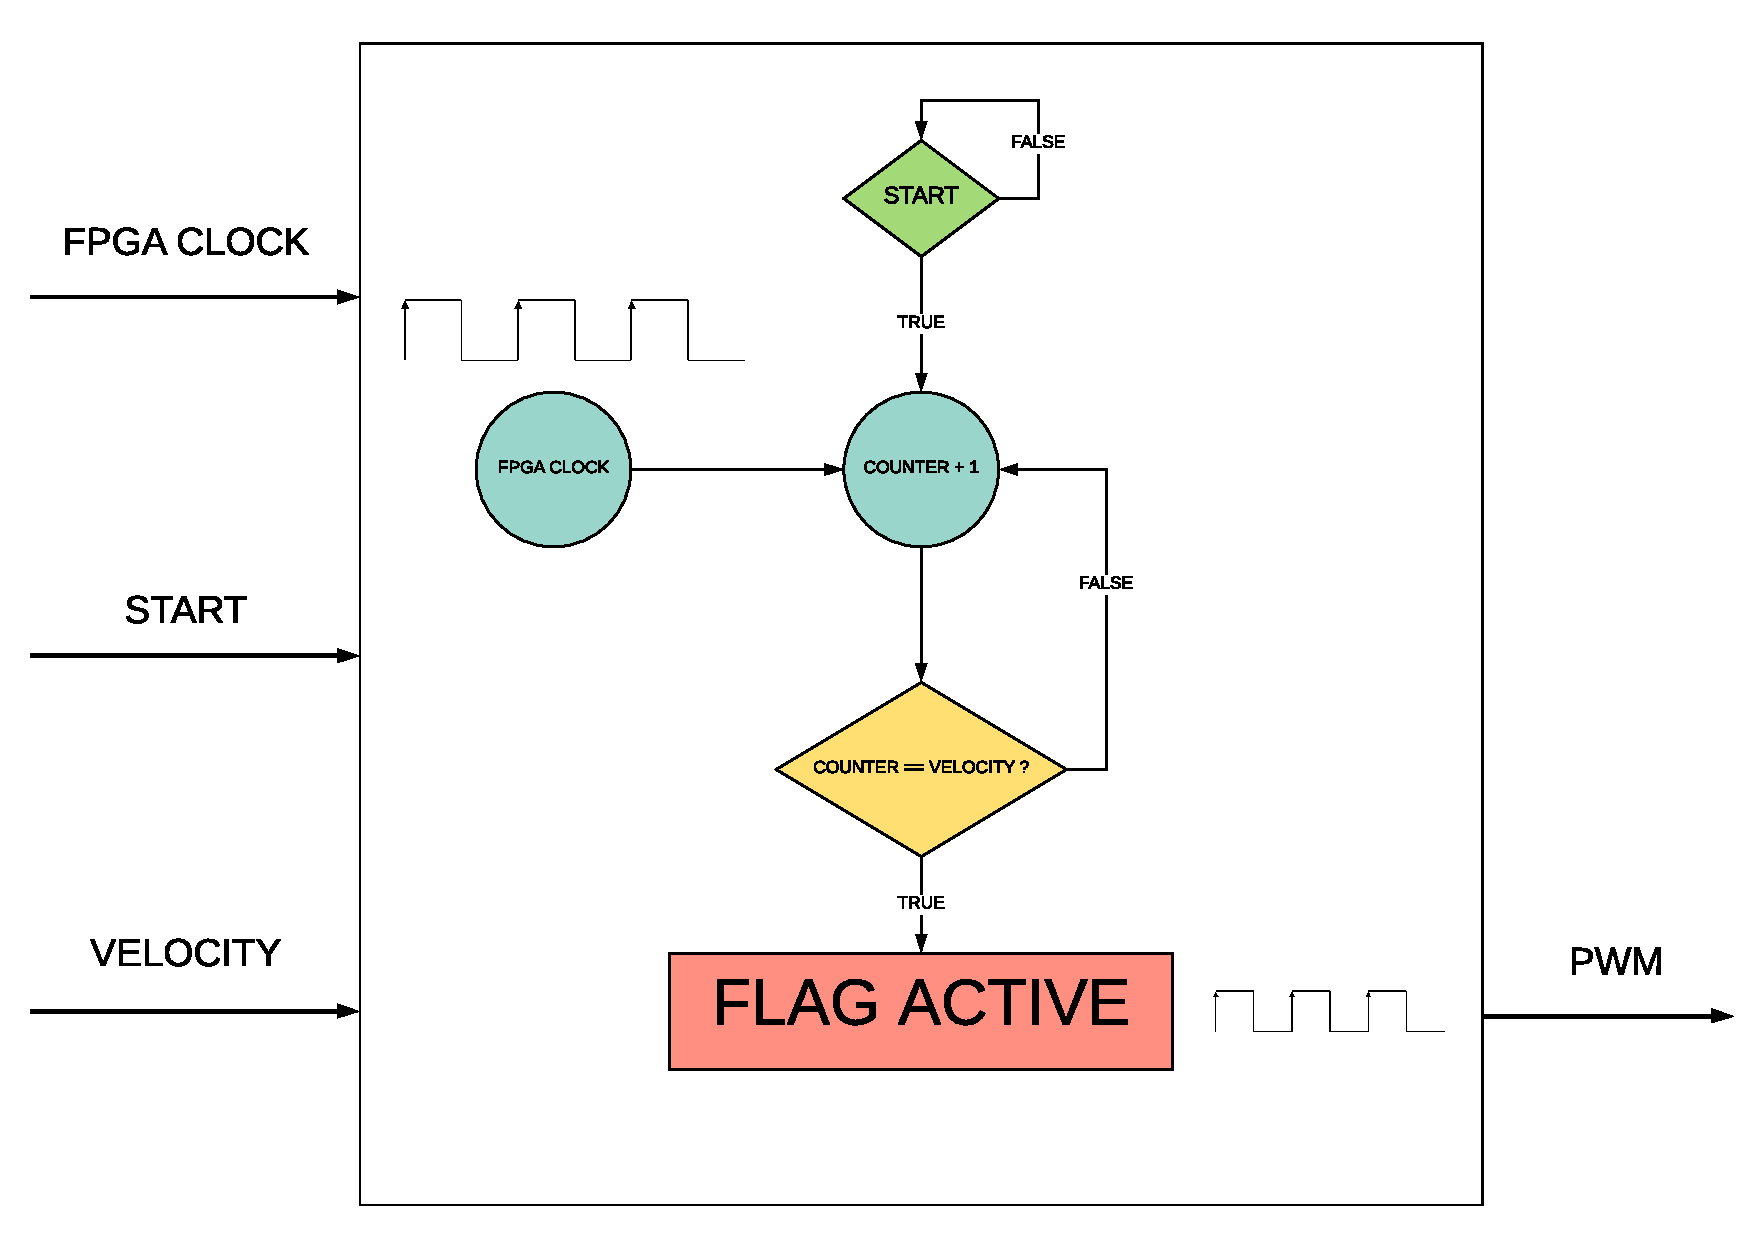
\includegraphics[trim = 0mm 0mm 0mm 0mm, clip,scale=0.6]{imagenes/Balancing_robot/pwm_control.pdf}
	\caption{Envío de ángulo usando el puerto serie.}
	\label{fig:pwm_control}
\end{figure}

\subsection{Sistema de alimentación}

Como todo sistema electrónico, es necesario una fuente de alimentación que permita el correcto funcionamiento de todos los componentes.  \newline
Se diferencia para ello dos subsistemas independientes en cuánto a la alimentación se refiere:
\begin{itemize}
	\item Alimentación para los motores DC.
	\item Alimentación de la propia tarjeta IceZum Alhambra II.
\end{itemize}

\subsubsection{Alimentación de los motores DC:}
Para la alimentación de los motores DC se hace uso de una batería LIPO de 11.1V y 2200maH como en la figura \ref{fig:lipo111}.

\begin{center}
	\begin{figure}[H]
		\center
		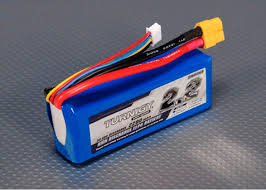
\includegraphics[scale=0.8]{imagenes/Balancing_Robot/LIPO111}
		\caption{Batería LIPO 11.1V y 2.2A. }
		\label{fig:lipo111}
	\end{figure}
\end{center}

\subsubsection{Alimentación IceZum Alhambra II:}

Para la alimentación de la IceZum Alhambra II se hace uso de una batería LIPO de 3.7V y 4mAh como la de la figura \ref{fig:lipo37}. 
\begin{center}
	\begin{figure}[H]
		\center
		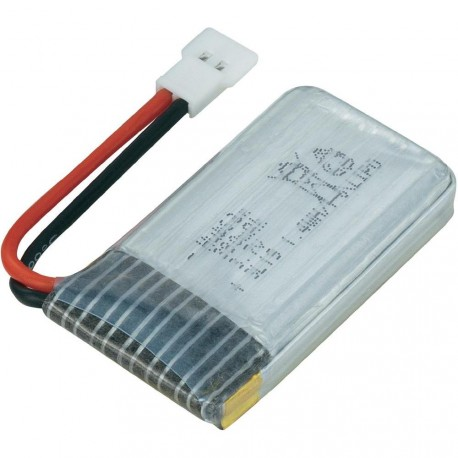
\includegraphics[scale=0.5]{imagenes/Balancing_Robot/LIPO37}
		\caption{Batería LIPO 3.7V y 4mAh.}
		\label{fig:lipo37}
	\end{figure}
\end{center}




y como tarea fundamental, un análisis de requerimientos de dichos componentes que forman el sistema completo es prioritario para poder elegir una alimentación adecuada. Además se tiene en cuenta que la finalidad es tener un sistema móvil y que en la medida de lo posible se evita una conexión directa a la red eléctrica o una conexión usb a un ordenador. Así, solo queda elegir que tipo de batería es adecuada. \newline

A continuación se nombran los diferentes tipos de bleatería con los se cuenta actualmente en el mercado analizando sus ventajas e inconvenientes más importantes: 

\begin{itemize}
	\item Baterías de plomo ácido. Son económicas y fáciles de fabricar pero no admiten sobrecargas ni descargas profundas, además, son de un peso y volumen muy elevados para la poca energía que son capaces de almacenar.
	\item Baterías de niquel-cadmio (Ni-Cd). Funcionan bien en un rango amplio de temperaturas, y se pueden sobrecargar sin sufrir daños. Admiten descargas profundas y proporcionan un buen número de ciclos. Como en la anterior, tienen un peso y volumen muy elevado.
	\item Baterías de niquel-hidruro metálico (Ni-MH). Mejora las características de las anteriores, sin embargo, proporciona un número menos de ciclos.
	\item Baterías de iones de litio (Li-ion). En comparación con las anteriores estas son de un desarrollo mas reciente y han facilitado la existencia de tecnologías portátiles. Tienen una capacidad elevada en relación a su peso y volumen, tienen un factor de auto-descarga muy elevado. Casi no se ven afectadas por el efecto memoria y pueden cargarse sin haber sido descargadas previamente. En contrapartida, no soportan bien los cambios de temperatura. 
	\item Baterías de polímero de litio (Li-Po). Son una variación de las baterías de Li-on que mejoran sus características de peso y volumen así como su tasa de descarga. Quedan prácticamente inutilizadas si se descargan en exceso.
\end{itemize}

Teniendo en cuenta cuál tiene que el sistema final y más restrictivo es un vehículo aéreo remotamente pilotado y que el balancing-robot necesita de un peso no muy elevado, es importante que las características de peso, volumen, y descarga sean las adecuadas. Por ello se elije para la alimentación de los sistemas en este proyecto las baterías de tipo Li-po, las cuáles pueden almacenar gran cantidad de energía y ofrecen una tasa de descarga muy alta. \newline

Las baterías de tipo Li-Po tienen una nomenclatura diferente del resto, la cuál es necesario analizar:

\begin{itemize}
	\item Clasificación por número de celdas "S". El número S corresponde con el número de celdas, las cuáles son de 3,7 voltios pero pueden llegar a 4,2 si están totalmente cargadas. Una batería de 3 celdas (3S) está compuesta por tanto de 3 sub-baterías puestas en serie, es decir, un total de 11,1 voltios.
	\item Capacidad indicada en "mAh". A mayor de número de miliamperios hora más capacidad de carga. Un error común es pensar que a mayor capacidad mas posibilidad de alargar el tiempo del sistema en cuestión. A mayor capacidad, el peso y volumen de la batería aumenta, por lo que hay que encontrar la mejor configuración para nuestro sistema. 
	\item Tasa de descarga "C". El número C corresponde con la tasa de descarga de la batería. Si una batería es de 1C significa que la máxima tasa de descarga a la que puede llegar es a la que se corresponde a su capacidad. Si el número C es distinto de 1 significa que multiplicamos la tasa de descarga por ese valor, reduciendo el tiempo de descarga proporcionalmente, esto es, una batería de 1000mAh 2C se descargaría a 2A en media hora.
\end{itemize}

El siguiente planteamiento sería por tanto elegir qué valores anteriores necesita nuestro sistema, para ello se desarrolla la siguiente tabla con los requerimientos de cada componente:

\begin{table}[H]
	\begin{tabular}{lllll}
		\hline
		\multicolumn{1}{|l|}{Componente}           & \multicolumn{1}{l|}{Voltaje de operación} & \multicolumn{1}{l|}{Corriente de salida por canal} & \multicolumn{1}{l|}{Canales de motor} & \multicolumn{1}{l|}{PWM máximo} \\ \hline
		\multicolumn{1}{|l|}{MC33926 Motor Driver} & \multicolumn{1}{l|}{5V-28V}               & \multicolumn{1}{l|}{2.5 A}                         & \multicolumn{1}{l|}{2}                & \multicolumn{1}{l|}{20kHz}      \\ \hline
		&                                           &                                                    &                                       &                                 \\
		&                                           &                                                    &                                       &                                
	\end{tabular}
\end{table}

\subsection{Materiales y coste del prototipo}
En la tabla \ref{tabla:coste} se desglosa el coste total del prototipo del sistema planteado.
\renewcommand\tablename{Tabla}
\begin{table}[H]
	\begin{tabular}{|l|l|l|l|l}
		\cline{1-4}
		\multicolumn{1}{|c|}{\cellcolor[HTML]{FFCE93}\textbf{MATERIAL}} & \cellcolor[HTML]{FFCE93}\textbf{CANTIDAD} & \multicolumn{1}{c|}{\cellcolor[HTML]{FFCE93}\textbf{\begin{tabular}[c]{@{}c@{}}COSTE \\ UNITARIO (€)\end{tabular}}} & \multicolumn{1}{c|}{\cellcolor[HTML]{FFCE93}\textbf{\begin{tabular}[c]{@{}c@{}}COSTE \\ TOTAL (€)\end{tabular}}} &  \\ \cline{1-4}
		IceZum Alhambra II                                              & 1                                         & 60                                                                                                                  & 60                                                                                                               &  \\ \cline{1-4}
		Arduino Nano                                                    & 1                                         & 8                                                                                                                   & 8                                                                                                                &  \\ \cline{1-4}
		Separador Hexagonal Nylon 10 mm                                 & 4                                         & 0.20                                                                                                                & 0.80                                                                                                             &  \\ \cline{1-4}
		Separador Metálico Hexagonal M3 25 mm                           & 8                                         & 0.25                                                                                                                & 2                                                                                                                &  \\ \cline{1-4}
		Separador Metálico Hexagonal M3 50 mm                           & 4                                         & 0.41                                                                                                                & 1.64                                                                                                             &  \\ \cline{1-4}
		Tornillo Nylon M3                                               & 16                                        & 0.09                                                                                                                & 1.44                                                                                                             &  \\ \cline{1-4}
		Tuerca Nylon M3                                                 & 8                                         & 0.05                                                                                                                & 0.40                                                                                                             &  \\ \cline{1-4}
		Tornillo Nylon M1                                               & 4                                         & 0.09                                                                                                                & 0.39                                                                                                             &  \\ \cline{1-4}
		Tuerca Nylon M1                                                 & 8                                         & 0.05                                                                                                                & 0.40                                                                                                             &  \\ \cline{1-4}
		Placa de Circuito Impreso 4 capas                               & 1                                         & 5                                                                                                                   & 5                                                                                                                &  \\ \cline{1-4}
		Rueda 7 cm                                                      & 2                                         & 7.90                                                                                                                & 15.80                                                                                                            &  \\ \cline{1-4}
		Motor DC                                                        & 2                                         & 24.95                                                                                                               & 49.9                                                                                                             &  \\ \cline{1-4}
		Driver Motor DC Dual MC33926                                    & 1                                         & 30                                                                                                                  & 30                                                                                                               &  \\ \cline{1-4}
		IMU MPU6050                                                     & 1                                         & 2.50                                                                                                                & 2.50                                                                                                             &  \\ \cline{1-4}
		Estructura mecánica 3D                                          & 1                                         & 20                                                                                                                  & 20                                                                                                               &  \\ \cline{1-4}
		Screw 3.5 mm                                                    & 5                                         & 0.80                                                                                                                & 4                                                                                                                &  \\ \cline{1-4}
		Cable 5-pin                                                     & 1                                         & 0.82                                                                                                                & 0.82                                                                                                             &  \\ \cline{1-4}
		Regleta PIN 2,54 mm 4 contactos Macho                           & 1                                         & 0.08                                                                                                                & 0.08                                                                                                             &  \\ \cline{1-4}
		Regleta PIN 2,54 mm 8 contactos Shield                          & 2                                         & 0.54                                                                                                                & 1.08                                                                                                             &  \\ \cline{1-4}
		Regleta PIN 2,54 mm 6 contactos Shield                          & 2                                         & 0.58                                                                                                                & 1.16                                                                                                             &  \\ \cline{1-4}
		Jumper 2.54 mm Puente de conexión                               & 2                                         & 0.08                                                                                                                & 0.16                                                                                                             &  \\ \cline{1-4}
		Regleta PIN 2,54 mm 10 contactos Hembra                         & 2                                         & 0.10                                                                                                                & 0.20                                                                                                             &  \\ \cline{1-4}
		Regleta PIN 2,54 mm 10 contactos Macho                          & 5                                         & 0.10                                                                                                                & 0.50                                                                                                             &  \\ \cline{1-4}
		Resistencia 4K7 5\%                                             & 3                                         & 0.21                                                                                                                & 0.63                                                                                                             &  \\ \cline{1-4}
		Estaño                                                          & 1                                         & 5.50                                                                                                                & 5.50                                                                                                             &  \\ \cline{1-4}
		Metro de cinta Termoretráctil                                   & 2                                         & 1.50                                                                                                                & 3                                                                                                                &  \\ \cline{1-4}
		Metro de cable 12 AWG                                           & 1                                         & 0.90                                                                                                                & 0.90                                                                                                             &  \\ \cline{1-4}
		Batería Lipo 11.1 V 2200 mA                                     & 1                                         & 19.95                                                                                                               & 19.95                                                                                                            &  \\ \cline{1-4}
		Batería Lipo 3.7 V 5 mA                                         & 1                                         & 4.20                                                                                                                & 4.20                                                                                                             &  \\ \cline{1-4}
		\multicolumn{2}{|c|}{}                                                                                      & \multicolumn{2}{c|}{\cellcolor[HTML]{FD6864}}                                                                                                                                                                                          &  \\
		\multicolumn{2}{|c|}{\multirow{-2}{*}{\textbf{COSTE TOTAL PROTOTIPO:}}}                                     & \multicolumn{2}{c|}{\multirow{-2}{*}{\cellcolor[HTML]{FD6864}\textbf{240.45}}}                                                                                                                                                         &  \\ \cline{1-4}
	\end{tabular}
	\caption{Coste total del prototipo Balancing-Robot.}
	\label{tabla:coste}
\end{table}

\section{Experimentos}
\subsection{VGA Module}
\subsection{Protocolo I2C}
\subsection{Controlador motor burshless}